\documentclass[a4paper,openright,12pt]{report}

\usepackage[spanish]{babel}
\usepackage{afterpage}
\usepackage{amssymb}
\usepackage{float}
\usepackage{algpseudocode}
\usepackage{algorithm}
% \usepackage[linesnumbered,algoruled,boxed,lined,spanish,onelanguage]{algorithm2e}
\usepackage[paper=A4,pagesize]{typearea}
\usepackage{longtable}
\usepackage{xcolor}
\usepackage{enumitem}
\usepackage{amsmath}
\usepackage{mathtools}
\usepackage{fancyvrb}
\usepackage{fixltx2e}
\usepackage{hyperref}
\usepackage[T1]{fontenc}
\usepackage[utf8]{inputenc}
\usepackage{graphicx}
\usepackage{apacite}
\usepackage[autostyle]{csquotes}
\usepackage{framed}
\usepackage{titlesec}
\usepackage[list=true]{subcaption}
\usepackage{url}
\usepackage{hyperref}


\setcounter{secnumdepth}{5}

\hypersetup{
    colorlinks,
    citecolor=blue,
    filecolor=blue,
    linkcolor=black,
    urlcolor=blue
}

\hyphenation{re-no-ván-do-se}
\hyphenation{e-le-men-to}
\hyphenation{ra-di-ca-les}
\hyphenation{con-lle-va-rí-a}
\hyphenation{ma-ni-pu-la-dos}
\hyphenation{de-sa-rro-llar}
\hyphenation{res-pec-to}

\urlstyle{same}
\setlength{\parskip}{1em}

% Support older LaTeX versions.
\DeclareUnicodeCharacter{2060}{}

% Parameter
% \makeatletter
% \g@addto@macro{\@algocf@init}{\SetKwInOut{Parameter}{Parámetro}}
% \makeatother
% Global
% \makeatletter
% \g@addto@macro{\@algocf@init}{\SetKwInOut{Global}{Global}}
% \makeatother



\makeatletter
\renewcommand{\ALG@name}{Algoritmo}
\renewcommand{\algorithmicrequire}{\textbf{Entrada: }}
\renewcommand{\algorithmicensure}{\textbf{Salida: }}
\renewcommand{\algorithmicfor}{\textbf{para}}
\renewcommand{\algorithmicdo}{\textbf{hacer}}
\renewcommand{\listalgorithmname}{Lista de \ALG@name s}
\makeatother

\algdef{SE}[SUBALG]{Indent}{EndIndent}{}{\algorithmicend\ }%
\algtext*{Indent}
\algtext*{EndIndent}

\algdef{SE}[PARAMETERS]{Parameters}{EndParameters}
   {\algorithmicvariables}
   {\algorithmicend\ \algorithmicvariables}
\algnewcommand{\algorithmicvariables}{\textbf{parámetros}}



\begin{document}
\begin{titlepage}
	\centering

	{\sffamily\large\bfseries PONTIFICIA UNIVERSIDAD CATÓLICA DEL PERÚ \par}
	\vspace{0.2cm}
	{\sffamily\large\bfseries INGENIERÍA INFORMÁTICA\par}
	\vfill

	
\includegraphics[width=6cm]{../images/logo-pucp.png}\par\vspace{1cm}
	\vspace{1.5cm}

	{\sffamily\large\bfseries Implementación de un plug-in para GStreamer para
	el seguimiento de rostros aplicado a Cheese\par}
	\vspace{2cm}

	{\sffamily\small Tesis para optar por el título de Ingeniero Informático que
		presenta el bachiller: }

	{\sffamily\Large\bf	César Fabián Orcccón Chipana \par}
	{\sffamily 20105515 \par}
	\vfill
	{\sffamily Asesor: Dr.~Ivan \textsc{Sipiran} \par}

	\vfill

% Bottom of the page
	{\sffamily\large \today\par}
\end{titlepage}



\tableofcontents
\chapter{Generalidades}
\section{Problemática}


Por más de 130 años las personas han usado cámaras para documentar sus vidas
\cite{snap2017prospectus}.
Cuando las primeras cámaras fueron inventadas, era difícil y costoso tomarse una
fotografía \cite{snap2017prospectus}. Un filtro fotográfico es un accesorio para las
cámaras fotográficas que se inserta en la parte frontal de esta para conseguir
cierto efecto deseado. La historia de los filtros fotográficos también es muy
antigua, y se remonta al siglo XIX. En 1878, Frederick Wratten, un innovador e
investigador del campo de la fotografía introdujo un proceso conocido como
“noodling” que permitía crear placas fotográficas más sensitivos que las
existentes en esa época \cite{hannavy2013encyclopedia}⁠. En 1906, él junto con
su hijo y el doctor C. E. Kenneth
Mees fundaron una compañía llamada Wainwright Ltd., en la cual Mees ayudó a
Wratten a desarrollar las primeras placas pancromáticas y los primeros filtros
de luz, los cuales se harían conocidos como Wratten filters
\cite{hannavy2013encyclopedia}⁠. Kodak compraría
más tarde Wainwright Ltd. en el 1912 \cite{hannavy2013encyclopedia}⁠. Desde
entonces, los filtros fotográficos han ganado popularidad, y renovándose hasta
la actualidad.\\

En las dos últimas décadas, la aparición de la fotografía digital ha dejado
atrás a las cámaras de película \cite{CIPAfilmCameraStats}. En la actualidad,
es común contar si no con una cámara digital, entonces al menos con una cámara
web integrada al computador personal portátil o al telefóno inteligente. El
término “filtro” (el cual de aquí y en
adelante será entendido como “filtro digital”) también se ha mudado al contexto
digital y se ha introducido en el hablar del común de muchas personas. Las
razones por las cuales las personas aplican filtros a sus fotografías son
varias. Algunos aplican filtros para mejorar la estética regulando el brillo,
contraste y focalización \cite{bakhshi2015we}. Otros desean aplicar efectos
antiguos, por ejemplo algunos colocan las fotografías en blanco y negro para
concentrar la atención en cierta textura de la toma y evitar que el espectador
se distraiga en los colores, otros simplemente desean darle un aspecto de
antigüedad \cite{bakhshi2015we}. Otras personas simplemente desean cambiar los
colores \cite{bakhshi2015we}. Finalmente, algunos otros simplemente
desean darle un aspecto único y divertido a las fotografías
\cite{bakhshi2015we}. El único propósito de estos últimos es el agregar
características divertidas (a través de filtros) que no pudieron ser capturadas
originalmente por la cámara \cite{bakhshi2015we}.\\

Hoy en día, diversas empresas se han apalancado del fácil acceso a la cámara web
por parte de los usuarios de teléfonos inteligentes destacando entre ellas
empresas como Skype Technologies S.A.R.L (Skype), Oath Inc. (Flickr),
Facebook Inc. (Facebook e Instagram) y Snap Inc. (Snapchat) han permitido la
edición de imágenes aplicando filtros de manera sencilla para sus usuarios. Por
ejemplo, la aplicación para móviles Snapchat se ha hecho muy popular por no solo
aplicar filtros que permiten regular los colores de la foto o video en tiempo
real, sino que permite detectar objetos capturados por la cámara del dispositivo
y seleccionar entre una diversa variedad de lentes que permite sobreponer
animaciones interactivas sobre la toma \cite{snap2017prospectus}⁠. Este tipo de
filtros se han popularizado especialmente entre “millennials”. Por ejemplo, para
Snapchat, los jóvenes de entre 18 y 24 años representan un 36\% de sus usuarios
activos por día en Estados Unidos \cite{snap2017prospectus}⁠. De hecho, muchos
jóvenes adultos sostienen que este tipo de filtros resuelve problemas de
comunicación dado en ciertas redes sociales debido a que la sobreposición de
imágenes y texto puede clarificar el mensaje que ellos desean expresar en sus
fotografías \cite{vaterlaus2016snapchat}. El deseo por agregar imágenes sobre
las fotografías, no se limita a occidente. De hecho, esta práctica ha sido y es
muy común en Japón desde la década de los noventas. En el año 1995, Altus, una
empresa japonesa, desarrolló un fotomatón (un quiosco para tomarse fotos,
generalmente insertando una moneda) que permitía agregar pegatinas sobre las
fotografías \cite{edwards2004photographs}. Atlus patentó una máquina con el
nombre de Purikura, término que se volvería más adelante en un término del uso
cotidiano de las personas en Japón principalmente los adolescentes
\cite{edwards2004photographs}. Recientemente, estas máquinas también se han
renovado incluyendo filtros digitales para el agregado de imágenes sobre las
fotografías \cite{TheOrigi29}.\\

En las computadoras de escritorio, podemos dividir la situación actual de las
aplicaciones de webcam por el Sistema Operativo en los cuales están soportadas.
Por un lado, en macOS, la aplicación para capturar fotos y videos con la cámara
web por defecto es Photo Booth, la cual permite aplicar filtros en tiempo real,
así como detectar a una persona para reemplazar el fondo por un video
preestablecido o foto colocada manualmente por el usuario \cite{photoBooth}. Fun
Booth es una aplicación para macOS. desarrollada por Spoonjuice LLC, la cual
permite detectar un rostro humano frente a la cámara para colocar imágenes sobre
este \cite{funBooth}. Por otro lado, Windows 10 incluye una aplicación para la toma de fotos y grabación de
video, pero esta no dispone de filtros tan sofisticados como los de Photo Booth.
Sin embargo, existen aplicaciones de terceros con varias funcionalidades.
CyberLink YouCam, de CyberLink Corp. permite no solo detectar el rostro del
individuo capturado y sobreponer filtros sobre esto, sino que detecta las
emociones de las personas \cite{YouCam7A82}⁠. ManyCam que entre diversas
funcionalidades que ofrece, permite además aplicar filtros para colocar máscaras
y animaciones que rastrean el rostro de la persona ubicada frente a la webcam
\cite{Webcamso75}. Para sistemas operativos basados en GNU/Linux, existen
programas que permiten ajustar los colores de las capturas con la cámara web,
pero la aplicación, al parecer, más popular y a la vez con filtros más
sofisticados es Cheese, proyecto de la GNOME Foundation \cite{AppsChee13}.⁠\\

Cheese, a diferencia del resto de programas mencionados con licencia privativa,
es un software libre \cite{cheeseLicense}⁠. El software libre a diferencia del software privativo,
según la Free Software Foundation, es el software que respeta la libertad de sus
usuarios y comunidad permitiéndoles tener el derecho de ejecutar, copiar,
distribuir, estudiar, modificar y mejorar el programa \cite{whatIsFreeSoftware}⁠.
Cheese está licenciado bajo la licencia GNU General Public License versión 2
(GPLv2) \cite{cheeseLicense}⁠.
El hecho de que este tenga una licencia libre es fundamental para el desarrollo
de este proyecto de fin de carrera, pues permite a otros estudiar su código
fuente, mejorarlo y modificarlo. Este software, además, ha sido financiado por
Alphabet Inc. en varias ocasiones. De hecho, este fue inicialmente desarrollado
en el 2007 por Daniel G. Siegel como parte de un proyecto del Google Summer of
Code (GSoC), programa ideado por Larry Page y Sergey Brin, fundadores de Google,
para difundir el software libre y de código abierto remunerando a estudiantes
por desarrollar en este tipo de proyectos \cite{gsoc1}.\\


La necesidad por agregar soporte para sobreposición de imágenes sobre el rostro
de las capturas de Cheese fue expresado en el 2010 ⁠\cite{Bug6279256} y, además
ya hubo intentos de agregar esta funcionalidad. En el GNOME Outreach Program for
Women (programa para mujeres similar al GSoC pero financiado por la GNOME
Foundation, ahora llamado Outreachy) del 2010, la participante Laura Elisa Lucas
Alday, trabajó en desarrollar un filtro (elemento) para GStreamer, un framework
especializado en el procesamiento multimedia, llamado gstfaceoverlay, el cual
permitía la adición de imágenes en formato svg sobre un rostro detectado en una
imagen \cite{faceoverlay}\cite{gopw1}. El filtro fue aceptado por los
desarrolladores GStreamer, y posteriormente agregado a GNOME Video Effects,
librería que contiene una lista de filtros o combinación de filtros de GStreamer
en archivos de texto y que son usados por Cheese para aplicar los filtros. Sin
embargo, este filtro fue posteriormente retirado de GNOME Video Effects puesto
que algunos archivos svg hacían lento (el “framerate” caía) a Cheese
\cite{Bug6641489}.\\


En setiembre 2012, GStreamer 1.0 fue lanzado, y desde esa fecha, gstfaceoverlay
no fue portado a la nueva versión de GStreamer. Esto llevó a que el filtro fuera
borrado de la librería el 21 de diciembre del 2016. Ante esto, en el 2016, se
propuso un parche en el ``bug tracker'' de GNOME para portar el filtro a las
series GStreamer 1.x, el cual sería aceptado en GStreamer en el año 2017
\cite{Bug7640127}. Una vez portado, se probó su funcionamiento en Cheese
\cite{CFOCHfunnyStickersCheese} y se observó que además de solo soportar la
sobreposición de imágenes con formato SVG, este filtro no puede detectar el
rostro de más de una persona. Ello condujo a proponer otro parche que solucione
este problema \cite{Bug7691771}. Sin embargo, esta solución si bien al parecer
es correcta en un contexto aislado, arrastra un problema en su base. El problema
fundamental en este filtro es que no ha debido implementarse sobre la base del
filtro gstfacedetect, otro filtro para GStreamer especializado en la detección
de rostros. De hecho, usar gstfacedetect como base es un error si se
desea usar el plugin en Cheese para dar soporte a múltiples rostros con
múltiples imágenes, pues este aplica la detección facial para cada cuadro (o
\textit{“frame”} en inglés), pero sin respetar un orden alguno, es decir que una
persona etiquetada en el primer cuadro con la imagen A podría ser etiquetada en
el segundo marco con la imagen B, y en el tercero otra vez con A o tal vez con
C. Lo esperado sería que si se sobrepuso la imagen A sobre el rostro de una
persona, esta imagen A se mantenga sobrepuesta en los siguientes cuadros.\\

Para conseguir que Cheese soporte filtros de sobreposición de imágenes sobre los
rostros de personas en tiempo real no es suficiente escribir un nuevo filtro
para GStreamer. Tampoco es suficiente, luego de escribir el filtro, agregar la
configuración del “pipeline” de GStreamer a GNOME Video Effects de tal modo que
Cheese pueda leerlo. Cheese debería implementar una interfaz gráfica en la cual
el usuario pueda seleccionar e importar imágenes que desea usar, de este modo
se evita el uso de efectos estáticos predeterminados. Es preciso resaltar que
realizar tales cambios a Cheese no es fácil para nuevos colaboradores del
proyecto. Cheese no se ha actualizado recientemente, y una de las razones puede
ser que existe pocas personas que sepan programar en Vala, un lenguaje de
programación orientado a objetos con un compilador que traduce el
código a C para compilarlo compilado con gcc \cite{valaOverview}. Además Cheese
usa Clutter \cite{CheeseDependencyClutter}, librería de GNOME basada en OpenGL,
para mostrar la salida de la captura y los efectos aplicados en la pantalla.
Ambos no disponen de mucha documentación disponible pública, y por lo general,
uno debe guiarse en base a otros programas que han sido escritos usando tanto
Clutter como Vala. Por otro lado, entre los filtros a usar para el rastreamiento
de imágenes, algunos como face4d no tienen licencias compatibles con GPLv2, para
lo cual no solo es necesario escribir software libre, sino que el código debe
ser compatible con esta licencia.\\

En conclusión, se puede observar que los usuarios de software para la cámara web
tienen varias razones para preferir usar filtros. El problema es más acentuado para
usuarios de software libre. Los programas de escritorio con licencias libres o
de código abierto para capturar imagen y video están quedándose atrasados
tecnológicamente. Sin embargo, el problema no solo está en este tipo de software,
sino que pareciera que las aplicaciones para macOS también están en la misma
situación. Recientemente, la aparición de Snapchat ha creado una tendencia entre
millennials de 18 a 24 años a tener una preferencia por filtros que sobreponen
imágenes que siguen sus rostros capturados por la cámara web a otros medios
de comunicación convencionales. Siendo Cheese un software libre, lo cual
representa una ventaja social sobre el software privativo, es posible estudiarlo
y mejorarlo (sin mencionar otras libertades) puede ser considerado como la mejor
opción para implementar la característica de sobreposición de imágenes sobre
cuadros capturados por la webcam, ya que tiene mejores características que otros
proyectos de software libre similares para escritorio. Agregar la funcionalidad
de aplicar filtros que sobrepongan imágenes sobre los rostros de las personas
capturados por una webcam en tiempo real no solo es beneficio para los jóvenes
millennials, sino también para la GNOME Foundation y podría aumentar la
competitividad entre aplicaciones de escritorio de captura de video y entre
entornos de escritorio para sistemas basados en UNIX (incluyendo macOS).

\section{Objetivos}
\subsection{Objetivo general}
Implementar e integrar en Cheese un plugin para GStreamer que mediante el uso de
algoritmos para detección y seguimiento de múltiples rostros (o una adaptación
de estos) permita sobreponer imágenes sobre los rostros detectados en videos
(particularmente, por la cámara web).

\subsection{Objetivos específicos}
\subsubsection{OE0: Objetivo Específico 0}
Desarrollar un algoritmo e implementarlo como un filtro de GStreamer para
la detección y rastreamiento de múltiples rostros con soporte para oclusión
así como la detección de puntos faciales de la cara.
\subsubsection{OE1: Objetivo Específico 1}
Escribir el código fuente de un filtro para GStreamer que basado en el filtro
implementado en \textit{OE1} permita la sobreposición de imágenes sobre puntos
predeterminados en los rostros detectados.
\subsubsection{OE2: Objetivo Específico 3}
Diseñar una interfaz gráfica para Cheese que permita al usuario de Cheese
aplicar el filtro implementado en \textit{OE2}.

\subsection{Resultados esperados}
\subsubsection{REOE0: Resultados esperados para el Objetivo Específico 0}
Un filtro que implemente un algoritmo de rastreo de múltiples rostros, siendo
este algoritmo propio o una implementación de alguno existente. Este filtro
definirá una estructura o interfaz donde se guardarán las coordenadas de los
rostros y sus puntos puntos faciales. Esta interfaz servirá como medio de
comunicación entre el filtro y otros filtros o entre el filtro y la aplicación
final. Además este filtro debe ser personalizable para regular el desempeño del
filtro y por ende mejorar el delay.
\subsubsection{REOE1: Resultados esperados para el Objetivo Específico 1}
Un filtro que tomando como referencia las coordenadas de diversos puntos de cada
rostro detectado ofrezca un conjunto parámetros de entrada para colocar imágenes
en lugares predefinidos del rostro como filtrum (parte entre la boca y nariz),
boca, ojos, nariz, orejas y cara.
\subsubsection{REOE2: Resultados esperados para el Objetivo Específico 2}
Una interfaz gráfica con un conjunto de imágenes clasificadas por categoría. De
estas imágenes el usuario puede seleccionar una o más de estas imágenes las
cuales serán sobrepuestas en los rostros detectados aplicando el filtro del
\textit{OE2}.

\subsection{Mapeo de objetivos, resultados y verificación}

A continuación se presenta la siguiente tabla para facilitar la identificación
de objetivos específicos, resultados y medios de verificación.

\begin{center}
  \begin{longtable}{| p{.4\linewidth} | p{.2\linewidth} | p{.3\linewidth} |}
  \hline

  % Row
  \multicolumn{3}{|p{\linewidth}|}{Objetivo (\textit{OE0}): Desarrollar un algoritmo que
  implemente un filtro para \textit{GStreamer} para la detección y rastreamiento
  de múltiples rostros con soporte para oclusión y detección de puntos faciales.}
  \\ \hline

  \textbf{Resultado} &
  \textbf{Meta física} &
  \textbf{Medio de verificación}
  \\ \hline

  Filtro para \textit{GStreamer} que permita el rastreamiento de rostros y
  detección de puntos faciales del rostro a partir de un modelo entrenado 
  permitiendo regular el retardo ajustando parámetros. &
  Software &
  \textit{Precision}, \textit{recall}, \textit{accuracy} y
  \textit{F1 score} del detector y rastreador de rostros, y comparación del
  \textit{latency} creado entre el filtro existente y el desarrollado.
  \\ \hline

  % Row
  \multicolumn{3}{|p{\linewidth}|}{Objetivo (\textit{OE1}): Escribir el código
  fuente de un filtro para GStreamer que basado en el filtro implementado en
  \textit{OE0} permita la sobreposición de imágenes sobre puntos predeterminados
  en los rostros detectados.}
  \\ \hline

  \textbf{Resultado} &
  \textbf{Meta física} &
  \textbf{Medio de verificación}
  \\ \hline

  Filtro para \textit{GStreamer} para sobreponer imágenes sobre las coordenadas
  detectadas. &
  Software &
  \textit{Latency} y pruebas unitarias de partes importantes del código.
  \\ \hline

  % Row
  \multicolumn{3}{|p{\linewidth}|}{Objetivo (\textit{OE2}): Diseñar una interfaz
  gráfica para Cheese que permita al usuario de Cheese aplicar el filtro
  implementado en \textit{OE1}.}
  \\ \hline

  \textbf{Resultado} &
  \textbf{Meta física} &
  \textbf{Medio de verificación}
  \\ \hline

  Filtro para \textit{GStreamer} para sobreponer imágenes sobre las coordenadas
  detectadas. &
  Software
  \\ \hline
  \end{longtable}
\end{center}



\subsection{Herramientas, métodos y procedimientos}

\subsubsection{En relación al Objetivo Específico 0 (OE0)}

\paragraph{Metodologías para detección de rostros}
\subparagraph{Metodología 0: Detector de objetos de Viola-Jones}\mbox{} \\
Este es el método que el filtro existente de \textit{GStreamer} llamado
\textit{gstfacedetect} que se usa actualmente. Este método basado en aprendizaje
de máquina para detectar objetos y procesar imágenes de manera muy rápida. Tres
principales contribuciones se brindan:

\begin{enumerate}
    \item \textbf{Imagen integral y vector de características tipo Haar}:
    la imagen integral (figura \ref{fig:integral-image-input} y
    \ref{fig:integral-image-output}) es manera de representar una imagen
    la cual se usa para generar un vector de características tipo Haar
    \cite{violajones}. Por ejemplo, si se tiene el rostro de una persona
    (figura \ref{fig:haar-face}), y se tiene dos rectángulos
    (figura \ref{fig:haar-face-with-rectangles}), el vector característica se
    puede calcular substrayendo la imagen integral del rectángulo negro con la
    imagen integral del rectángulo blanco \cite{wang2014analysis}.

    % Figura: Ejemplo de imagen integral.
    \begin{figure}[H]
      \begin{subfigure}[b]{0.4\textwidth}
        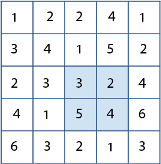
\includegraphics[width=0.6\textwidth]{../images/integral-image-input.png}
        \caption{Imagen de entrada.}
        \label{fig:integral-image-input}
      \end{subfigure}
      \hfill
      \begin{subfigure}[b]{0.4\textwidth}
        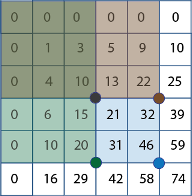
\includegraphics[width=0.6\textwidth]{../images/integral-image-output.png}
        \caption{Imagen integral.}
        \label{fig:integral-image-output}
      \end{subfigure}
      \caption{Ejemplo de imagen integral. La imagen integral siempre tendrá
      su primera columna y primera fila llena de ceros. Luego las demás celdas
      se calcula como la suma de los acumulados de las celdas anteriores.}
      \caption*{Imágenes tomadas y adaptadas de \cite{IntegralImageMathworks}}
    \end{figure}

    % Figura: Ejemplo de haar-like features
    \begin{figure}[H]
      \begin{subfigure}[b]{0.4\textwidth}
        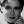
\includegraphics[width=0.5\textwidth]{../images/haar-face1.png}
        \caption{Imagen de un simple rostro en escalas grises.}
        \label{fig:haar-face}
      \end{subfigure}
      \hfill
      \begin{subfigure}[b]{0.4\textwidth}
        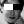
\includegraphics[width=0.5\textwidth]{../images/haar-face2.png}
        \caption{Rectángulos sobre los cuáles se calculará la imagen integral.}
        \label{fig:haar-face-with-rectangles}
      \end{subfigure}
      \caption{Ilustración de técnica usada para calcular los vectores de
      características tipo Haar. Una vez calculados la imagen integral en el
      rectángulo negro y blanco, estos se restan. El proceso se repite para
      todos los subrectángulos posibles y algunos métodos incluyen la rotación
      de estos.}
      \caption*{Imágenes tomadas de \cite{wang2014analysis}
      }
    \end{figure}

    \item \textbf{Entrenamiento con  Adaboost}: 
    Se usa una variante de Adaboost para descartar una gran cantidad de vectores
    característica, ya que tan solo usar un rectángulo de 24 x 24 píxeles crea
    162336 vectores característica \cite{wang2014analysis}.
    Lo que se busca es seleccionar los vectores característica más
    representativos \cite{violajones}. De esta manera se puede seleccionar una
    característica de 180000 posibles características \cite{violajones}.

    \item \textbf{Cascadas}:
    Se usa un árbol de decisiones llamado "cascada" \cite{violajones}.
    Se divide el clasificador en varios clasificadores \cite{violajones}.
    Un resultado positivo en un clasificador dispara otro clasificador, y así
    sucesivamente \cite{violajones}. Si un clasificador arroja un resultado
    negativo, la región rectangular ("subventana") es descartada
    \cite{violajones}. Cada clasificador consecutivo se conoce como
    \textit{stage}, y la ventana que pasa todos los \textit{stages} es una
    región de rostro \cite{violajones}.

    \begin{figure}[H]
      \centering
        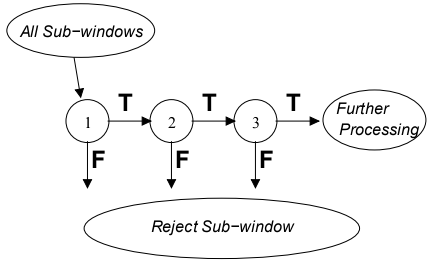
\includegraphics[width=0.7\textwidth]{../images/cascade-diagram.png}\par
      \caption{Diagrama de cascadas con 3 \textit{stages}. Cada subventana, un
      trozo de imagen que se desliza por la imagen a analizar, es pasada por
      este clasificador. Las ventanas que pasan satisfactoriamente el
      clasificador se consideran rostros.}
      \caption*{Fuente: \cite{violajones}}
      \label{fig:cascades-diagram}
    \end{figure}
\end{enumerate}

\subparagraph{Metodología 1: Histograma de gradientes para detección humana}\mbox{} \\
Este método se basa en la creación de vectores característica a partir de la
concatenación de desriptores de histogramas de gradientes. Según la publicación
original, el primer paso es aplicar una normalización gamma (o corrección
gamma). Esta suele ser usada para ajustar el brillo de las imágenes. Sin
embargo, los resultados de la publicación muestran que la ganancia es mínima
\cite{dalal2005histograms}.\\

Una vez preprocesada la imagen con el filtro gamma, se toma una porción de la
imagen (una ventana) la cual será filtrada con el kernel
$[\begin{matrix}-1 & 0 & 1\end{matrix}]$ y el kernel
$[\begin{matrix}-1 & 0 & 1\end{matrix}]^T$ \cite{dalal2005histograms}.
El resultado de aplicar este filtro son dos matrices en la que cada una
representa una aproximación a las derivadas parciales en $x$ y $y$.
Por tanto, dadas las derivadas parciales en ambas coordenadas se puede calcular
su magnitud y dirección. Estas dos matrices son, posteriormente usadas para
formar el histograma de gradientes el cual tiene un rango de
$[0^\circ, 180^\circ]$ y está formado por 9 \textit{bins}
\cite{dalal2005histograms}.\\

El histograma de gradientes generado es un vector característica de una celda
de $8 \times 8$ píxeles \cite{dalal2005histograms}. Ya que se usan bloques de
$16 \times 16$ píxeles, entonces se tiene 4 celdas de $8 \times 8$ píxeles
\cite{dalal2005histograms}. Por tanto, por cada celda se tiene un vector
característica de 9 componentes y si se concatena los 4 vectores se tendría un
vector en 36-D. Debido a que la iluminación o contraste puede influir 
en los valores de los vectores, este vector concatenado de 36 componentes es
normalizado \cite{dalal2005histograms}. De la misma manera, deslizando el
bloque de $16 \times 16$ por toda la imagen se va generando vectores
característica los cuales combinados (concatenados) dan un vector característica
final \textit{dalal2005histograms}.\\
Finalmente, para un conjunto de imágenes positivas (imágenes que contienen el
objeto a detectar, en este caso rostros) y para un conjuto de imágenes negativas
(que no contienen el objeto a detectar) se calcula los vectores característica
de ambos. Estos son pasados a un clasificador \textit{SVM}
\textit{dalal2005histograms}.

\paragraph{Metodologías y algoritmos para el seguimiento de rostros}\mbox{} \\
Según Zaheer Shaik y Vijayan Asari, los métodos de seguimiento de personas
pueden ser clasificados en cuatro categorías según la forma, las características,
el modelo o color de piel de la cara \cite{shaik2007robust}. Estos se detallan
a continuación:

\begin{enumerate}
    \item Seguimiento basado en la forma: en este método se debe usar un modelo
    que represente la locación de una cara. Se toma la elipse como el modelo más
    simple que mejor se ajusta a la forma de una cara \cite{eleftheriadis1995automatic}. Este método de
    seguimiento no es influenciado por el color de fondo ni por los cambios en
    la iluminación \cite{shaik2007robust}. Sin embargo, este falla si la cara rastreada es ocluida ya
    sea por otro objeto u otra persona \cite{shaik2007robust}.
    \item Seguimiento basado en características:  en este método, las
    características de los rostros son extraídas usando el filtro de Gabor el
    cual es usado como característica para el seguimiento de rostros \cite{shaik2007robust}. Sin
    embargo, este método no es sensible a los cambios en iluminación y la pose
    de la cara \cite{shaik2007robust}. Hacer que este método soporte esta característica tiene un alto
    costo computacional por lo que no es adecuado para streaming.
    \item Seguimiento basado en el modelo: este usa un modelo en 3D del rostro,
    el cual es proyectado en los cuadros detectados por la cámara \cite{shaik2007robust}. Sin embargo,
    estos pueden tener dificultad cuando hay cambios de iluminación o si la cara
    es ocluida \cite{smolyanskiy2014real}. Si bien esta metodología suele ser precisa tiene el problema de
    tener un alto costo computacional por lo que no es adecuado para streaming.
    \item Seguimiendo en base a los colores: este método usa el modelo de color
    de piel \cite{shaik2007robust}. Sin embargo, aunque falla cuando el rostro es ocluido, es adecuado
    para streaming.
\end{enumerate}

A continuación se describirán algunos métodos y algoritmos usados para el
seguimiento de rostros , de los cuales el proyecto puede potencialmente tomar
referencia en algunas partes o en su totalidad para implementar el filtro de
rastreo de rostros.

\subparagraph{Metodología 0: A Real-time Model for Multiple Human Face Tracking
              from Low-resolution Surveillance Videos}\mbox{} \\

Es un método propuesto por Rajib Sarkara, Sambit Baksh y Pankaj K Sa. Ha sido
probado en 1000 imágenes elegidas al azar de la base de datos de rostros
frontales de personas de Europa, Asia y África \cite{sarkar2012real}.
Su exactitud es del 96.2\% \cite{sarkar2012real}.
Además, con imágenes con resolución reducida a través de interpolación este
algoritmo tiene un comportamiento más eficiente \cite{sarkar2012real}.
A continuación se describen los pasos que sigue:
\begin{enumerate}[label=(\alph*)]
    \item Detectar y segementar las regiones de piel en una imagen
        \cite{sarkar2012real}. Para ello se usa el siguiente algoritmo:
    \begin{framed}
    \textbf{Entrada}: Una imagen $I$ en el modelo de color \textit{RGB} de
    dimensión.\\
    \textbf{Salida}: Una imagen binaria $S$ indicando si un pixel es piel o no.\\
    \textbf{Pasos}:\\
        \begin{enumerate}[label=\arabic*.]
            \item Convertir la imagen $I$ de \textit{RGB} a
                \textit{YC\textsubscript{b}C\textsubscript{r}}.
            \item Calcular la luma promedio de una imagen $I$ calculado como
                \[
                    {}_{I}Y_{prom} = {\sum_{i=1}^{m}\sum_{i=1}^{n} {}_{I}Y_{i,j}} 
                \]
            \item Normalizar ${}_{I}Y_{i,j}$ a ${[0,255]}$
            \item Encontrar el mapa de contornos usando el detector de bordes de
                Canny para la imagen de entrada \textit{RGB}.
            \item Encontrar la imagen compensada de brillo ${}_{I}C'$ obtenido
                de la siguiente manera:\\
                \textit{Cada pixel}
                    ${}_{I}C'_{i,j} = \{{}_{I}R'_{i,j}, {}_{I}G'_{i,j}, {}_{I}B'_{i,j}\}$
                \textit{donde:}\\
                \[
                    {}_{I}R'_{i,j} = ({}_{I}R'_{i,j})^\tau
                    {}_{I}G'_{i,j} = ({}_{I}G'_{i,j})^\tau
                    {}_{I}B'_{i,j} = ({}_{I}B'_{i,j})^\tau
                \]
                \textit{para:}
                \begin{equation}
                    \tau=
                    \begin{cases}
                        1.5, & \text{if }\ {}_{I}Y_{prom}<64\\
                        0.7, & \text{if }\ {}_{I}Y_{prom}>190\\
                        1
                    \end{cases}
                \end{equation}
            \item El mapa de colores de piel para ${}_{I}C'_{i,j}$ es calculado
                como:
                \begin{equation}
                    S_{i,j}=
                    \begin{cases}
                        0, & \text{if $\frac{R + 1}{G + 1}>1.08$ y $\frac{R + 1}{B + 1}>1.08$ y $G>30$ y $G<140$}\\
                        1
                    \end{cases}
                \end{equation}
                donde $S_{i,j}=0$ indica una región de piel y $S_{i,j}=0$ lo contrario.
        \end{enumerate}
        \raggedleft\cite{sarkar2012real}
    \end{framed}

    \item Verificar si cada componente de la piel corresponde (o no) a un
        rostro verificando la existencia de la boca y ojos \cite{sarkar2012real}.
    \item Colocar un cuadro en cierta orientación sobre la región de piel
        detectada dependiendo de la forma de la cara \cite{sarkar2012real}.
\end{enumerate}

\subparagraph{Metodología 1:
              A Robust Method for Multiple Face Tracking Using Kalman Filter}\mbox{} \\

Es un método propuesto por Zaheer Shaik y Vijayan Asari para el seguimiento de
múltiples rostros. Este resuelve el problema de oclusiones parciales y totales 
tomando como referencia el modelo de la ropa de las personas \cite{shaik2007robust}. Además también
supera los problemas de iluminación y cambios en las poses, velocidades y
trayectorias de los rostros \cite{shaik2007robust}. A continuación se describe la metodología empleada 
en más detalle.\\

Cada rastreador de rostro se inicia usando el algoritmo de detección de rostros
de Viola-Jones el cual se provee en \textit{OpenCV}, además se inician las
plantillas (\textit{templates} en inglés) de los rostros \cite{shaik2007robust}. Las caras detectadas
se limitan por un ROI (o región de interés) rectangular \cite{shaik2007robust}.
En este instante, también se inicia el modelo
de ropa que se usará para cada persona al cual corresponde a una función de
distribución de densidad no paramétrica \cite{shaik2007robust}. Como la distribución, de antemano, no
es conocida se usa una estimación de densidad (\textit{kernel}) tomando como
\textit{kernel} la función de Epanechnikov \cite{shaik2007robust}. De esta manera, la función de
distribución de la ropa para una región $q_{u}$ se calcula de la siguiente
manera:
\[
    q_{u} = C{\sum_{i,j} k(\lVert x_{ij} \rVert^2)\delta[b(x_{ij}) - u]}
\]
donde $\delta$ es la función de Kronecker, $k$ el \textit{kernel} de
Epanechnikov y $b$ es la función que asocia un pixel $x$ en la posición $ij$
a un índice $b(x_{ij})$ en un espacio de colores cuantificada (es decir en un
espacio de colores reducido) \cite{shaik2007robust}. Esta función representa
la probabilidad de que un píxel con valor $u$ en una región $q$, en este caso
la ropa.\\

Además se usa el filtro de Kalman, el cual es un filtro usado para la estimación
de ciertas variables en el futuro con aplicaciones en predicción de análisis
financieros, navegación y control de vehículos, procesamiento de señales,
econometría y seguimiento de gráficos interactivos por computadora
\cite{bishop2001introduction}. Para ello, se usan cinco variables: $x_{t}$ 
y $y_{t}$ que corresponden a la posición de la esquina superior izquierda de los
rectángulos que bordean los rostros detectados, $y'_{t}$ y $y'_{t}$ que
representan las velocidades, y por último, el ancho del rectángulo $W_{t}$
\cite{shaik2007robust}. La altura no se considera, pero se asume igual a $1.25$
veces el ancho \cite{shaik2007robust}. A continuación se muestra el modelo de
estados usado (siendo las variables con sufijo ${t + 1}$ las coordenadas
predichas y $w_{t}$ el ruido gausiano):
\[
    \begin{bmatrix}
        x_{t+1}\\
        y_{t+1}\\
        x'_{t+1}\\
        y'_{t+1}\\
        W_{t+1}
    \end{bmatrix}
    =
    \begin{bmatrix}
        1   &   0   &   \Delta{t}   &   0           &   0\\
        0   &   1   &   0           &   \Delta{t}   &   0\\
        0   &   0   &   1           &   0           &   0\\
        0   &   0   &   0           &   1           &   0\\
        0   &   0   &   0           &   0           &   1\\
    \end{bmatrix}
    \begin{bmatrix}
        x_{t}\\
        y_{t}\\
        x'_{t}\\
        y'_{t}\\
        W_{t}
    \end{bmatrix}
    +
    w_{t}
\]
Estas variables predichas se usan para localizar un rostro en el frame
actual \cite{shaik2007robust}. Usando una técnica de coincidencia de plantillas o (\textit{template
matching} en inglés), se calcula la distancia entre la plantilla de una cara del
cuadro anterior y de la región con los valores predichos \cite{shaik2007robust}. Si el cuadro anterior
es menor a un \textit{threshold} de 0.9, se asume \textbf{oclusión parcial} \cite{shaik2007robust}.
Además basándose en las coordenadas para el cuadro ``actual'' halladas por el
filtro de Kalman, se recalcula el modelo de distribución de la ropa para el
cuadro actual ($p_{u}$) \cite{shaik2007robust}. Luego se debe medir la similitud entre las
distribuciones $q_{u}$ y $p_{u}$ \cite{shaik2007robust}. Para ello se usa la métrica estadística
conocida como la distancia de Bhattacharyya la cual es dada por
$\rho = \sum_{u}\sqrt{(p_{u}.q_{u})}$ \cite{shaik2007robust}. Si $\rho$ es menor que un
\textit{threshold} de 0.5, se asume que los modelos no son similares y deben de
ser actualizados \cite{shaik2007robust}.\\
Para actualizar el \textit{template} de rostro se debe redetectar los rostros en
el frame actual \cite{shaik2007robust}. Para ello, se usa una técnica basada en los colores \cite{shaik2007robust}. Tomando el
espacio de color cuantificado (reducido), se busca clasificar los pixeles como
``tipo piel'' o ``no tipo piel'' \cite{shaik2007robust}. Para ello se usa el espacio de color
\textit{YC\textsubscript{b}C\textsubscript{r}}, en el cual la luma \textit{Y} es
separada: ello hace este algoritmo robusto a cambios en la iluminación. Luego,
estos pixeles son clasificados como piel según un threshold en los rangos de
$[100,135]$ y $[135,170]$ para C\textsubscript{b} y C\textsubscript{r},
respectivamente \cite{shaik2007robust}. Una vez identifacadas las regiones de piel, se agrupan los
pixeles de una región para la detección del rostro \cite{shaik2007robust}. La primera etapa consiste en
erosionar la imagen de la región de la cara usando una elipse, para luego
erosinarlas con el fin de llenar los huecos dejados entre los rostros. El
resultado es una máscara binaria de \textit{blobs} de las regiones de los
rostros \cite{shaik2007robust}.\\

Para detectar la región al rededor de cada \textit{blob} se usa un algoritmo
de detección de bordes el cual es implementado por \textit{OpenCV} \cite{shaik2007robust}. Luego, a los
contornos detectados se les aplica un parámetro estadístico llamado el
coeficiente de suavidad para cada ``blob'' \cite{shaik2007robust}. Si el coeficiente para un
\textit{blob} es menor a $0.5$, este se descarta \cite{shaik2007robust}.\\

En los \textit{blobs} restantes, se aplica un ``factor de forma'', el cual
relaciona el área entre el perímetro \cite{shaik2007robust}. Este se compara al ``factor de forma''
mínimo calculado para los primeros rectángulos que limitaban los rostros
detectados cuando se usó Viola-Jones \cite{shaik2007robust}. El fin de esto es eliminar más
\textit{blobs} \cite{shaik2007robust}. Luego para los \textit{blobs} que sobraron, se dibujan los
rectángulos tomando solo en consideración el ancho del \textit{blob} \cite{shaik2007robust}.\\

Una vez detectados los rostros, si el número de caras detectados es menor al
número de caras rastreadas, se asume oclusión total \cite{shaik2007robust}. Luego, si existe más
rostros de los clasificados como haber sido objetivo de rastreo en un cuadro
anterior, se dice que un nuevo rostros existe (por ejemplo, entra una nueva
persona a la zona de grabación) \cite{shaik2007robust}. Luego, la ecuación de medición del filtro de Kalman, se actualiza según:
\[
    \begin{bmatrix}
        mx_{t+1}\\
        my_{t+1}\\
        mW_{t+1}
    \end{bmatrix}
    =
    \begin{bmatrix}
        1   &   0   &   \Delta{t}   &   0           &   0\\
        0   &   1   &   0           &   \Delta{t}   &   0\\
        0   &   0   &   0           &   0           &   1\\
    \end{bmatrix}
    \begin{bmatrix}
        x_{t - \Delta{t}}\\
        y_{t - \Delta{t}}\\
        x'_{t - \Delta{t}}\\
        y'_{t - \Delta{t}}\\
        W_{t - \Delta{t}}
    \end{bmatrix}
    +
    v_{t}
\]
donde $mx_{t+1}$, $my_{t+1}$ y $mW_{t+1}$ corresponden a variables de medición,
y $v_{t}$ es el ruido de medición, representado por ruido gausiano \cite{shaik2007robust}. Así las
variables son actualizadas en el cuadro actual tomando el pasado (el cuadro
anterior) \cite{shaik2007robust}. Esto permite al algorimo seguir múltiples rostros de personas en el
caso de oclusión, variación de luz y el cambio de la pose \cite{shaik2007robust}.

\subparagraph{Metodología 3: Rastreamiento del landmark en un dispositivo móvil}
\mbox{} \\
Es un método para rastrear puntos faciales de la cara. Se toma como
objetivo de rastreo cinco puntos faciales: la parte externa de los ojos
izquierdo y derecho, punta de la nariz y esquinas del labio
\cite{wettum2017facial}. Véase la figura
la \ref{fig:landmark-tracking-5-keypoints}.\\

% Imagen de puntos faciales
\begin{figure}[H]
  \centering
    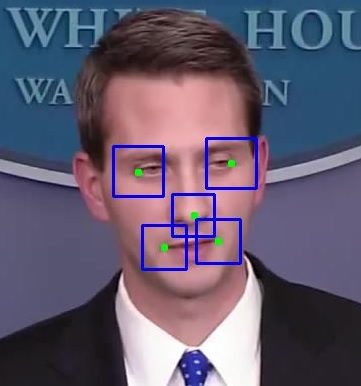
\includegraphics[width=0.3\columnwidth]{../images/landmark-tracking-1.png}\par
  \caption{Cada 50 \textit{frames} se detecta cinco puntos faciales del rostro y
    se inicializa un rastreador por cada punto facial con un \textit{ROI}
    (región de interés) cuyo tamaño es proporcional a la distancia interocular
    (distancia entre entre los ojos).}
  \caption*{Fuente: \cite{wettum2017facial}}
  \label{fig:landmark-tracking-5-keypoints}
\end{figure}

La técnica consiste en detectar dichos puntos en el primer cuadro
(\textit{frame}), luego desde el cuadro número 2 hasta el cuadro 50 se usa algún
rastreador tales como \textit{DFLD}, \textit{KCF}, \textit{DSST}, \textit{LK} o
\textit{Struck} \cite{wettum2017facial}. En el cuadro número 51, se vueleve a
detectar los puntos faciales para corregir, y así sucesivamente. Es decir,
cada 50 cuadros se detecta los puntos faciales y en las brechas cada uno de los
cinco rastreadores se encarga de rastrear sus respectivos puntos asignados
\cite{wettum2017facial}. Véase la figura \ref{fig:landmark-tracking-diagram}.\\

% Imagen de puntos faciales
\begin{figure}[H]
  \centering
    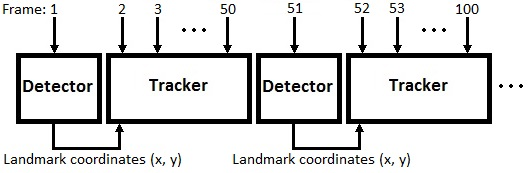
\includegraphics[width=0.5\columnwidth]{../images/landmark-tracking-2.png}\par
  \caption{Diagrama que muestra las alternaciones de detección y rastreo.}
  \caption*{Fuente: \cite{wettum2017facial}}
  \label{fig:landmark-tracking-diagram}
\end{figure}


\subparagraph{Metodología 3: Rastreamiento de múltiples objetos usando el
método húngaro y el filtro de Kalman}
\mbox{} \\

En un artículo académico, se desarrolló un sistema para el seguimiento y
clasificación de objetos (peces) en movimiento \cite{szHucs2015svm}. El primer
paso consiste en detectar los objetos, guardando sus regiones de interés con sus
respectivos \textit{timestamp}, las cuales serían entrada para el proceso de
clasificación \cite{szHucs2015svm}. Para la detección se usan diversos métodos,
los cuales no son de interés ya que su objetivo estaba enfocado en peces
\cite{szHucs2015svm}.\\

Luego de detectar los objetos, se usa el filtro de Kalman para rastrear los
objetos en los tres pasos básicos del filtro de Kalman: inicialización,
predicción y corrección \cite{szHucs2015svm}. En la etapa de inicialización,
se inicializa el filtro de Kalman por cada objeto detectado
\cite{szHucs2015svm}. En la etapa de predicción, se estimaba la posición del
objeto en el siguiente cuadro. En la etapa de corrección, se usa la información
de la medición de los objetos detectados para corregir los resultados de la
predicción del filtro \cite{szHucs2015svm}. Sin embargo, esto no era suficiente
por sí solo, y había que realizar un pareo entre los objetos detectados y para
ello se usó el método húngaro \cite{szHucs2015svm}.\\

Sea $v_{i}$ para $i \in 0...k$ un objeto rastreado en el cuadro actual, y sea
$w_{j}$ para $j \in 0...l$ el nuevo objeto detectado en el siguiente cuadro, el
primer paso es crear una matriz $M_{k \times l}$ donde cada celda de la matriz
$M[i,j]$ representa la distancia (euclideana) de $v_{i}$ a $w_{j}$
\cite{szHucs2015svm}. Las filas y columnas que superaban cierto límite
(\textit{threshold}) eran borradas para evitar un pareo (o asignación) erróneo
\cite{szHucs2015svm}. Si $v_{i}$ se removía significaba que el valor del
coeficiente de confianza (CFV) devía bajarse \cite{szHucs2015svm}. Si se removía
$w_{j}$, significaba que este objeto era probablemente un nuevo objeto y se
creaba un nuevo filtro de Kalman para este \cite{szHucs2015svm}.\\

% Imagen de puntos faciales
\begin{figure}[H]
  \centering
    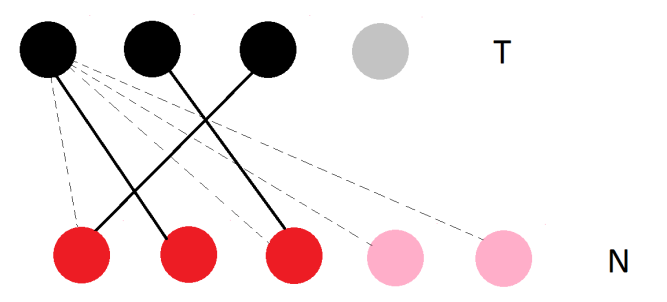
\includegraphics[width=1.0\columnwidth]{../images/hungarian-1.png}\par
  \caption{En la figura, los círculos negros y rojos representan los objetos
    rastreados en el cuadro actual y los objetos detectados en el siguiente
    cuadro, respectivamente. Luego de aplicar el método Húngaro, ciertos
    círculos negros son asignados a los círculos rojos. Los círculos con baja
    opacidad representan objetos que no fueron asignados, porque superaron el
    \textit{threshold}}
  \caption*{Fuente: \cite{szHucs2015svm}}
  \label{fig:hungarian-diagram-1}
\end{figure}

\paragraph{Herramientas empleadas}\mbox{} \\
\begin{enumerate}
    \item OpenCV, ya que implementa algunos algoritmos y técnicas
        útiles para el seguimiento y detección de objetos (rostros) y
        procesamiento de imágenes:
    \begin{enumerate}
        \item Conversión a espacios de color, usado para trabajar las imágenes
            RGB en distintos espacios de color entre estos \textit{GRAY} y
            \textit{YC\textsubscript{b}C\textsubscript{r}}.
        \item Proporciona una librería de rastreadores de rostros, entre ellos
            \textit{MIL}, \textit{Boosting}, \textit{Median flow}, \textit{TLD},
            \textit{KCF} y además implementa el filtro de Kalman.
        \item Erosión y dilatación de imágenes.
    \end{enumerate}
    \item \textit{GStreamer}, ya que es el framework sobre el cual se
        implementará el filtro.
    \item \textit{gstfacedetect}, filtro para \textit{GStreamer} que usa OpenCV
        para la detección de rostros y envía señales al \textit{bus} con las
        coordenadas localizadas.
    \item \textit{C++}, ya que OpenCV y GStreamer lo soportan.
    \item \textit{mesonbuild} es un sistema de compilación de código fuente muy
    rápido y fácil de usar a comparación que \textit{autotools}. De hecho, este
    sistema es el que se empieza a usar en muchos programas de \textit{GNOME}
    últimamente en reemplazo de \textit{autotools}.
    \item gst-launch-1.0, un programa para construir \textit{pipelines} de
    streaming de audio y video por línea de comandos, para probar manualmente
    la salida del streaming.
    \item Dlib, un \textit{toolkit} en \textit{C++} que proporciona algoritmos
    de machine learning, y que entre una de sus características está la de
    detectar el \textit{landmark} o puntos faciales de un rostro.
\end{enumerate}

\subsubsection{En relación al Objetivo Específico 1 (OE1)}
\begin{enumerate}
    \item \textit{gstcairooverlay}, un filtro para \textit{GStreamer} que usa
        la librería \textit{Cairo} la cual permite dibujar sobre las imágenes o
        cuadros recibidos por este filtro.
    \item \textit{vapigen}, para generar \textit{bindings} que permitan la
        compatibilidad entre el código escrito en \textit{C} y el código escrito
        en \textit{Vala}, el cual será usado para el siguiente objetivo.
    \item \textit{GStreamer}, \textit{C}, \textit{mesonbuild} y
        \textit{gst-launch-1.0} por las mismas razones mencionadas en el caso
        anterior.
\end{enumerate}

\subsubsection{En relación al Objetivo Específico 2 (OE2)}
\begin{enumerate}
    \item \textit{Gtk+}, librería para diseñar interfaces gráficas para GNOME,
        la cual es usada por \textit{Cheese} y se usará para diseñar la
        interfaz gráfica para seleccionar las imágenes a sobreponer sobre
        los rostros.
    \item \textit{Glade}, una interfaz gráfica en GTK+ para construir interfaces
        gráficas en GTK+.
    \item \textit{Vala}, lenguaje en el cual se desarrolla \textit{Cheese}.
    \item \textit{GStreamer}, integrando los filtros implementados con
        \textit{Cheese}.
    \item \textit{GLib Test Suite}, para ejecutar pruebas sobre el nuevo código
        agregado a \textit{Cheese}.
\end{enumerate}

\section{Alcance, limitaciones y riesgos}

\subsubsection{Alcance}
    Este proyecto se concentrará en funcionar en las computadoras por lo menos
    tres años antiguas con sistemas operativos GNU/Linux con entorno de
    escritorio \textit{GNOME}. Es decir, la detección, seguimiento y
    sobreposición de imágenes en Cheese debería dar la sensación de fluidez a
    usuarios de estas computadoras. Además, este proyecto debe funcionar sobre
    \textit{Wayland} ya que es el protocolo más usado recientemente por las
    distribuciones de GNU/Linux reemplazando a \textit{X.Org}
    \cite{LinuxMagazineWaylandStrong}.

\subsubsection{Limitaciones}
Se identifican las siguientes limitaciones:

\begin{enumerate}
    \item El desempeño del software desarrollado puede tener comportamientos
      distintos según la computadora en la cual se pruebe. Este puede ser
      afectado por diversos factores desde el retardo de la cámara web hasta la
      velocidad de procesamiento de la CPU.
    \item La aceptación del proyecto oficialmente en \textit{Cheese} depende de
      revisiones de terceros y del mantenedor de \textit{Cheese}, por lo que no
      se puede asegurar que el resultado será incluido oficialmente.
\end{enumerate}

\subsubsection{Riesgos}
Un proyecto de fin de carrera puede estar asociado a diversos riesgos. Los
riesgos listados en la tabla de abajo no solo implican situaciones del mismo
proyecto, sino también riesgos externos los cuales pueden afectar negativamente
el desarrollo de este proyecto.


\begin{center}
  \begin{longtable}{| p{.4\textwidth} | p{.15\textwidth} | p{.4\textwidth} |}
  \hline

  \textbf{Riesgo identificado} &
  \textbf{Impacto} &
  \textbf{Medidas para mitigar el riesgo}
  \\ \hline

  La brecha de seguridad, principalmente a través de un ataque cibernético por
  \textit{hackers} puede poner en riesgo cuentas donde se tiene publicados los
  avances del proyecto de fin de carrera. Estas amenazas puede incluir acceso
  no autorizado a cuentas como \textit{github}, \textit{Google Drive} y
  correo electrónico del autor del proyecto.&
  Medio&
  Mantener los avances del proyecto en más de una cuenta, y evitar limitarse
  a una sola cuenta.
  \\ \hline

  La aparición de \textit{blocker bugs} en actualizaciones de dependencias
  pueden impactar negativamente en el cumplimiento del cronograma previsto y
  además afectar la compatibilidad del software presentado con las últimas
  versiones en dependencias. &
  Bajo &
  Los \textit{blocker bugs} suelen ser temporales, por tanto, si en el
  transcurso del proyecto apareciera alguno, se debería reportar el \textit{bug}
  en caso de no estar reportado y simplemente esperar hasta que aparezca una
  actualización. Mientras tanto se deberá trabajar sobre una versión anterior
  de la dependencia.
  \\ \hline

  Actualizaciones y cambios radicales en las librerías como \textit{GStreamer},
  \textit{OpenCV} y \textit{dlib} que cambien la forma de trabajo puede retrasar
  el avance del desarrollo del software debido a que implicará un esfuerzo extra
  el aprender la nueva forma de uso de estos programas. &
  Bajo &
  Estar al pendiente de páginas, blogs, foros y listas de correos de las
  respectivas librerías con el fin de estar al tanto de las últimas
  actualizaciones con el fin de evitar de que el software use funciones
  obsoletas.
  \\ \hline

  \end{longtable}
\end{center}

\section{Justificación y viabilidad}

\subsection{Justificación}
Este proyecto se desarrolla por varias razones La primera, y la principal, es la
de entregar a las personas, y en especial a la comunidad de software libre, un
software le permita divertirse haciendo uso de la cámara web de su computadora
de escritorio sin tener que verse en la necesidad de recurrir a software
privativo o propietario, y por tanto respetando la libertad de su informática. Esta
manera de ``divertirse'' se desarrolla a través de la introducción de una mejora,
un filtro que permite sobreposicionar imágenes en la captura de la cámra web. En
un contexto social, donde prima los valores y ética, bajo ninguna razón se
debería desarrollar ni usar software privativo. Por un lado, cuando un
desarrollador licencia un programa con licencia privativa este automáticamente
toma control sobre sus usuarios. Sin embargo, el usuario, quien es el dueño de
la computadora, es quien debería tener el control de esta. Cuando un
desarrollador tiene el control este suele verse tentado a introducir de manera
intencional funcionalidades en los programas que dañan a sus usuarios actuando
en contra de sus intereses (\textit{malware}). Existe evidencia para calificar
a tanto el software de \textit{Apple, Inc} como el de \textit{Microsoft, Inc}
como malware \cite{malwareFSF} según la \textit{Free Software Foundation}.
Un ejemplo de ello es \textit{Skype} en el cual la NSA podía tener accesso a
los datos de los usuarios de Skype (tanto en video, voz, mensajes en texto y
archivos compartidos entre sus usuarios) \cite{skypeMalware}.
Por otro lado, el usuario de software privativo
constantemente cae en dilemas éticos: ¿quién debería decidir si compartir el
software: el usuario o el desarrollador? Si el mejor amigo de este usuario
pidiera una copia a su amigo, este tendría dos opciones: quedar bien con su
amigo copiando el software, pero actuando ilegalmente o no prestar el software
y quedar mal con su amigo \cite{patentesRMS}. Escribiendo software libre se
respeta la libertad del usuario. La segunda razón tiene como
propósito potenciar la creación y mejora de otros software multimedia que se
pueda apalancar de los filtros que quedarán como resultado de este proyecto.
Por ejemplo, algunos usuarios de \textit{Pitivi}, editor de video no lineal
basado en GStreamer, han solicitado que se agregue el mecanismo para poder
agregar parches sobre los rostros de personas en los videos. El filtro de
seguimiento de rostros implementado para \textit{Cheese} podría escanear los
rostros de diversos individuos a lo largo de un \textit{clip} de video en
\textit{Pitivi} y automáticamente generar \textit{keyframes} los cuales
indicarían la posición de múltiples parches sobre los rostros de las peronas y
que podrían ser manipulados o borrados simplemente agregando símbolos que
representen parches en el \textit{viewer} de \textit{Pitivi} los cuales pueden
ser arrastrados o borrados.

\subsection{Análisis de viabilidad}
\subsubsection{Viabilidad técnica}
Con respecto a la implementación del filtro en \textit{GStreamer}, si bien
desarrollar plugins para GStreamer tiene una curva de aprendizaje relativamente
larga, se tiene experiencia desarrollando tanto \textit{src pads} como filtros
para \textit{GStreamer}, por lo que desarrollar este filtro no sería un
problema. Con respecto a la implementación del algoritmo de rastreo de rostros,
se cuenta con los conocimientos fundamentales para poder implementarlos
satisfactoriamente, además se tiene la disposición de herramientas de código
abierto como \textit{OpenCV} y \textit{dlib} (sobre los cuales se ha realizado
experimentos previos), así como la disposición de un asesor quien domina el tema
de visión artificial. En cuanto a \textit{GTK+} y otras librerías de
GNOME, no solo se ha desarrollado anteriormente aplicaciones usando estas
tecnologías (\textit{Pitivi}), sino que incluso se ha aportado en el desarrollo
en proyectos como Libpeas y GObject, por lo que se tiene
conocimiento de algunas librerías a profundidad. En relación a los lenguajes a
usar \textit{Vala} y \textit{C++}, el primero tiene un parecido a \textit{C\#},
el cual ha sido enseñado en un curso de la universidad así como el segundo. Por
otra parte, en relación a \textit{Cheese}, además de tener a disposición el
código fuente, se ha intentado con anterioridad implementar la funcionalidad del
proyecto por lo que se conoce ciertas partes relevantes del programa, además se
tiene contacto directo con el actual mantenedor del proyecto \textit{Cheese},
David King, quien ha mostrado interés en el proyecto y ofrecido su ayuda incluso
para revisar el código.

\subsubsection{Viabilidad temporal}
La implementación del proyecto dará inicio el 11/12/2017 y se contará con tres
meses aproximadamente para tener la mayor parte del proyecto concluida. Los
siguientes cuatro meses (aproximados) se dedicará a realizar algunos ajustes, y
realizar la documentación requerida. A continuación, se muestra las tareas
identificadas que involucra cumplir con cada resultado esperado y el tiempo por
tarea estimado en horas.

\begin{center}
  \begin{longtable}{| p{.7\textwidth} | p{.25\textwidth} |}
  \hline

  \textbf{Tarea} &
  \textbf{Horas estimadas}
  \\ \hline

  \multicolumn{2}{| c |}{Completar el resultado esperado \textit{REOE0}}
  \\ \hline

  Preparar el \textit{dataset} &
  24
  \\ \hline

  Implementar alguna de las metodologías propuestas o una variación o
  combinación de estas \textit{GStreamer} en C++&
  144
  \\ \hline

  Agregar soporte para detección de los \textit{landmarks} usando \textit{dlib} &
  32
  \\ \hline

  Medir \textit{accuracy}, \textit{precision} y \textit{recall} &
  16
  \\ \hline

  Definir propiedades del objeto y estructura (\textit{GstStruct}) que se
  enviará al \textit{bus} &
  2
  \\ \hline

  Construir el \textit{Boilerplate} del plugin para \textit{GStreamer}
  incluyendo \textit{OpenCV} como dependencia &
  6
  \\ \hline

  Integrar el algoritmo implementado en un filtro de \textit{GStreamer} &
  60
  \\ \hline

  Medir \textit{accuracy}, \textit{precision} y \textit{recall} en el filtro&
  16
  \\ \hline

  Medir la latencia (\textit{latency}) del filtro o \textit{pipeline} &
  16
  \\ \hline

  \multicolumn{2}{| c |}{Completar el resultado esperado \textit{REOE1}}
  \\ \hline

  Definir propiedades del objeto &
  3
  \\ \hline

  Implementar filtro de sobreposición de imágenes &
  24
  \\ \hline

  Medir el retraso (\textit{latency}) agregado por el filtro &
  8
  \\ \hline

  \multicolumn{2}{| c |}{Completar el resultado esperado \textit{REOE2}}
  \\ \hline

  Diseñar \textit{mockups} de la interfaz gráfica&
  8
  \\ \hline

  Implementar interfaz gráfica en \textit{Cheese} para los filtros&
  24
  \\ \hline

  Integrar filtros del proyecto con el \textit{pipeline} de \textit{Cheese}&
  80
  \\ \hline

  Escribir \textit{unit tests} &
  16
  \\ \hline
  \end{longtable}
\end{center}

\subsubsection{Viabilidad económica}
Debido a que el proyecto se apalancará no solo de herramientas con licencias
de software libre sino que gratuitas, no se puede identificar costos fijos
relacionados en este aspecto. Se identifican costos fijos aunque menores
provenientes de la energía eléctrica y costos para un total de 500 horas de
trabajo aproximadas. También se debe precisar que este proyecto agregaría costos
relevantes de mantenimiento en caso de que las contribuciones sean oficialmente
aceptadas por \textit{The GNOME Project}.

\chapter{Marco Conceptual}
\section{Objetivos del marco conceptual}
A continuación se explicará algunos conceptos que se consideran básicos para
poder comprender los siguientes capítulos \cite{shaik2007robust}. En primer lugar, se explica qué es
el software libre ya que a veces es un concepto que suele ser confundido. Luego,
se introduce a GStreamer, librería en la cual Cheese se basa. Finalmente, se
muestra una visión en conjunto del flujo de datos multimedia en Cheese, así como
las librerías que se usarán para implementar los algoritmos de seguimiento de
rostros.

\section{Software libre}
El software libre es el software que respeta la libertad de sus usuarios y
comunidad. Según la Free Software Foundation, para que un programa
informático sea calificado de software libre, su licencia debe otorgar las
siguientes cuatro libertades:
\begin{framed}
\begin{quote}
\begin{itemize}
\item La libertad de ejecutar el programa como se desea, con cualquier propósito
(libertad 0).
\item La libertad de estudiar cómo funciona el programa, y cambiarlo para que
haga lo que usted quiera (libertad 1). El acceso al código fuente es una condición
necesaria para ello.
\item La libertad de redistribuir copias para ayudar a su prójimo (libertad 2).
\item La libertad de distribuir copias de sus versiones modificadas a terceros
(libertad 3). Esto le permite ofrecer a toda la comunidad la oportunidad de
beneficiarse de las modificaciones. El acceso al código fuente es una condición
necesaria para ello.
\end{itemize}
\raggedleft\cite{cuatroLibertades}
\end{quote}
\end{framed}
Si estas cuatro libertades no se cumplieran, el software se consideraría no
libre. Como se puede observar además, el término “precio” no se ha mencionado.
Por lo que el software libre no es un tema de precios, sino como se mencionó
inicialmente, de libertad, lo cual está relacionado directamente con un tema
ético \cite{cuatroLibertades}. Sin embargo, se aclara esto ya que muchos suelen
confundirlo con “freeware”.
\section{Software no libre o software privativo}
El software no libre también llamado software privativo es todo software que no
cumple alguna de las cuatro libertades del software libre, y por tanto no es
software libre \cite{gnuCategories}.
\section{GNOME}
Es un entorno de escritorio para distribuciones de GNU/Linux y BSD. Está
desarrollado por The GNOME Project, parte del proyecto GNU. GNOME es software
libre y está formado por una amplia variedad de proyectos más pequeños los
cuales están licenciados en su mayoría bajo las licencias GPL y LGPL. GNOME
está financiado por algunas empresas grandes como Google Inc. y Red Hat Inc
\cite{GNOMEFoundation}. Entre estos proyectos se encuentran librerías
importantes como un conjunto de librerías para la creación de programas para
el usuario final y programas para el usuario final como editores de texto como
un navegador de archivos, un emulador de terminal, navegadores web, clientes
IRC, programas gráficos para el control de versiones en Git, reproductores de
audio y video, visores de imágenes entre una lista de más de cien proyectos
\cite{GNOMEProjects}. GNOME es uno de lo escritorios libres más populares y
está traducido en más de 40 idiomas \cite{GNOMETranslationTeams}.

\section{GStreamer}
Es un proyecto de GNOME. GStreamer es una librería de código abierto y
multiplataforma escrita en C con bindings en varios otros lenguages de
programación y basada en GObject. GStreamer implementa un modelo de
“pipelines” que enlaza una serie de elementos, por ejemplo, demultiplexores,
decodificadores, multiplexores, filtros y codificadores \cite{GStreamerFeatures}.
Ello permite que cada elemento cumpla una tarea específica. GStreamer permite
la creación de aplicaciones multimedia y streaming. Para ejemplificar,
considerar el caso de la reproducción reproducción de un archivo con formato
ogg, se puede pasar el elemento a un elemento llamado gstfilesrc, donde este lee
el archivo por buffers y pasa un buffer a un demuxer que separa el audio del
video. Los buffers de audio van a un decodificador de Vorbis (códec de audio),
mientras que los buffers de video son pasados a un decodificador de Theora
(códec de vídeo).
Cada buffer de audio es pasado a un elemento que se encargará de pasar los datos
recibidos, por ejemplo, a PulseAudio. Cada buffer de video, por su parte, podría
ser enviado a Wayland. PulseAudio se encargaría de trasladar esos datos al
driver de audio para emitir la salida por el parlante y Wayland se encargaría
de mostrar el video en pantalla.
\subsection{Elemento (GstElement)}
Un elemento (GstElement) Es una abstracción sobre la cual se basan la mayoría de
objetos de GStreamer para construir un pipeline, el cual es una cadena de
objetos GstElement enlazados. Un GstElement puede tener una entrada y una o más
salidas. En un demultiplexor gstoggdemux por ejemplo, la entrada serían buffers
del archivo en formato ogg, y las salidas serían por un lado, el audio, y por
el otro lado el vídeo.\\
Existe tres tipos de elementos muy usados:\\
\subsubsection{Sources}
Son productores de datos, puede ser por ejemplo \textit{gstvideotestsrc} que
produce datos para videos de prueba; otro ejemplo, podría ser
\textit{gstfilesrc} que carga datos de un archivo. Los source elements solo
tienen un source pad.

\begin{figure}[h]
  \centering
    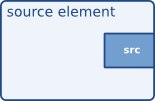
\includegraphics{../images/pwg-src-element.png}\par
  \caption{Representación de un \textit{source}}
  \caption*{Fuente: \cite[p.~5]{boulton2017gstreamer}}
\end{figure}

\subsubsection{Sinks}
Representan consumidores de datos. Por ejemplo, \textit{glimagesink} recibe
frames en un buffers y los renderiza usando OpenGL mostrando el resultado en una
ventana. \textit{waylandsink}, \textit{xvimagesink}, \textit{cluttersink}
cumplen roles similares pero usan internamente Wayland, X y Clutter
respectivamente. Un ``sink element'' solo tiene un sink pad.

\begin{figure}[h]
  \centering
    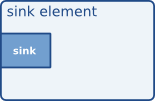
\includegraphics{../images/pwg-sink-element.png}\par
  \caption{Representación de un \textit{sink}}
  \caption*{Fuente: \cite[p.~5]{boulton2017gstreamer}}
\end{figure}

\subsubsection{Filtros}
Un filtro recibe ciertos datos, los procesa, y envía los datos modificados por
una o más salidas. Un ejemplo de filtro es agingtv que agrega un efecto de
televisión antigua. Otro ejemplo es \textit{glfiltercube} que usa OpenGL para
crear un cubo cuyas caras están texturizadas con los frames que este filtro
recibe. Un filtro tiene un source pad y un sink pad.

\begin{figure}[h]
  \centering
    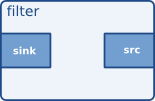
\includegraphics{../images/pwg-filter-element.png}\par
  \caption{Representación de un filtro}
  \caption*{Fuente: \cite[p.~5]{boulton2017gstreamer}}
\end{figure}

\subsubsection{Bin}
Un \textit{bin} es un tipo de elemento que contiene más elementos. La cantidad
de \textit{source pads} que posee y la cantidad de sink pads (ambos llamados
\textit{ghost pads} cuando se trata de un \textit{bin}) que posee puede ser
variable, y por lo general, depende de los elementos que están en sus extremos.

\begin{figure}[h]
  \centering
    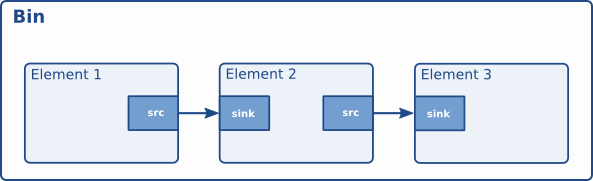
\includegraphics[width=\textwidth]{../images/ad-bin.png}\par
  \caption{Representación de un \textit{bin}}
  \caption*{Fuente: \cite{taymans2016gstreamer}}
\end{figure}


\subsubsection{Pipeline}
Es, por lo general, el bin de máximo nivel en una aplicación. Un
\textit{pipeline} controla el reloj (\textit{GstClock}) global del cual dispone
GStreamer, además dispone de un bus el cual controla, por lo que la aplicación
no tiene la necesidad de crear un bus. Un pipeline puede recibir consultas de
la aplicación como por ejemplo para hacer seeking o para obtener duración del
video reproducido con el pipeline.

\begin{figure}[h]
  \centering
    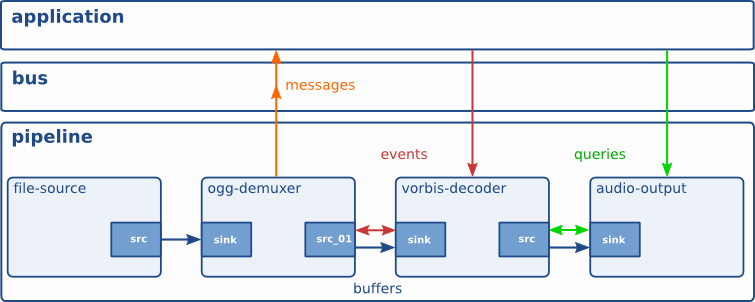
\includegraphics[width=\textwidth]{../images/ad-pipeline.png}\par
  \caption{Representación de un \textit{pipeline}}
  \caption*{Fuente: \cite{taymans2016gstreamer}}
\end{figure}

\subsection{Bus (GstBus)}
GStreamer es una librería multihilo. Cada GStreamer el bus es el encargado de
recibir mensajes del pipeline y enviarlos a la aplicación. La aplicación puede
capturar estos mensajes usando un \textit{callback} (similar a un
\textit{signal handler}). Por ejemplo, \textit{facedetect} usa \textit{OpenCV}
para detectar los rostros, y el tamaño y coordenadas de los rostros detectados
son enviadas al bus. De esta manera, una aplicación u otro elemento como
\textit{gstfaceoverlay} puede leer los mensajes en el bus y decidir qué hacer
con la información recibida, en este caso sobreponer imágenes.
\subsection{Plugin (GstPlugin)}
GStreamer es extendible a través de plugins. Un plugin puede contener uno o un
conjunto de elementos. Un plugin no es un elemento. En GStreamer, entre los
sets de plugins más populares se encuentran:
\begin{itemize}
\item \textbf{gst-plugins-base} es un set de plugins con los elementos esenciales para
la creación de elementos más complejos.
\item \textbf{gst-plugins-good} es un set de plugins soportado activamente por
la comunidad de GStreamer. Está licenciado bajo LGPL.
\item \textbf{gst-plugins-ugly} también licenciado bajo la licencia LGPL
(versión 2.1), es un set de plugins que puede carecer de revisiones, un
mantenedor activo, documentación, pruebas unitarias o cuyos desarrolladores
pueden tener dudas respecto a ciertas patentes.
\item \textbf{gst-plugins-bad} es un set de plugins que puede tener problemas
de distribución.
\end{itemize}
\section{Clutter}
Es una librería que usa OpenGL para crear interfaces gráficas ocultando la
complejidad de este mismo. Coloca a la disposición del desarrollador
herramientas para agregar texto, animaciones, imágenes los cuales, por ejemplo,
pueden ser arbitrariamente colocados o rotados \cite{clutterOverview}. Clutter
se integra tanto con Gtk como con Gstreamer.
\section{Vala}
Es un lenguaje de programación orientado a objetos desarrollado para adaptarse
mejor a las librerías de GNOME. El compilador de Vala es valac, el cual compila
código en Vala, generando archivos del lenguaje C, los cuales son compilados con
\textit{gcc}. La orientación a objetos está dada debido a que internamente usa
GObject, librería de GNOME que simula la programación orientada a objetos en C.
El hecho de que compilar programas escritos en Vala genere código fuente en C,
la necesidad de escribir bindings. Sintácticamente, es idéntico a C\#
\cite{valaOverview}.
\section{GNOME Video Effects}
Es una colección de filtros de GStreamer \cite{GNOMEVideoEffects} guardados en
archivos de texto con un título, una pequeña descripción y la descripción del
\textit{pipeline}.
\section{Cheese}
Es un proyecto de GNOME nacido en el 2007 como parte de un proyecto de Google
Summer of Code. Escrito inicialmente por el entonces estudiante Daniel G. Siegel
y mantenido actualmente por David King. Cheese es un programa para capturar
fotos y videos con la cámara web con la opción de aplicar filtros. Está
licenciado bajo la licencia GPLv2, y escrito principalmente en el lenguaje de
programación Vala, aunque con partes escritas en C \cite{cheeseReferenceManual}
\cite{cheeseApp}.\\

\begin{figure}
\begin{subfigure}{0.4\textwidth}
  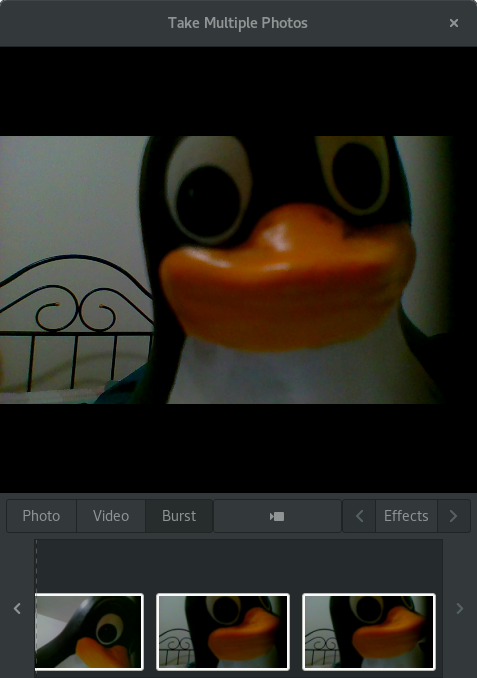
\includegraphics[width=\textwidth]{../images/cheese-viewport.png}
  \caption{Ventana principal de Cheese}
\end{subfigure}
\hfill\vrule\hfill
\begin{subfigure}{0.4\textwidth}
  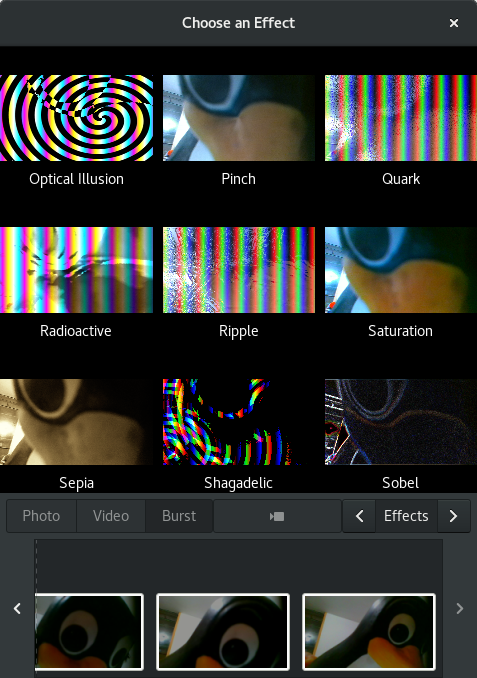
\includegraphics[width=\textwidth]{../images/cheese-effects-grid.png}
  \caption{Ventana de efectos de Cheese}
\end{subfigure}
\caption[Hello]{Cheese}
\caption*{Fuente: autoría propia}
\end{figure}

Cheese lee los filtros o efectos de GNOME Video Effects y los usa para
mostrarlos en su interfaz gráfica. Tanto la captura de videos (o fotos) como la
aplicación de filtros en Cheese está dada internamente por GStreamer, un
framework que permite el desarrollo de aplicaciones multimedia. Cheese crea
internamente una pipeline bastante compleja, de la cual se muestra una
simplificación en el diagrama de la \textit{figura 2.7}. El diagrama ignora
elementos como \textit{capsfilters}, \textit{bins} y algunos otros filtros y
elementos.

\begin{figure}
  \centering
    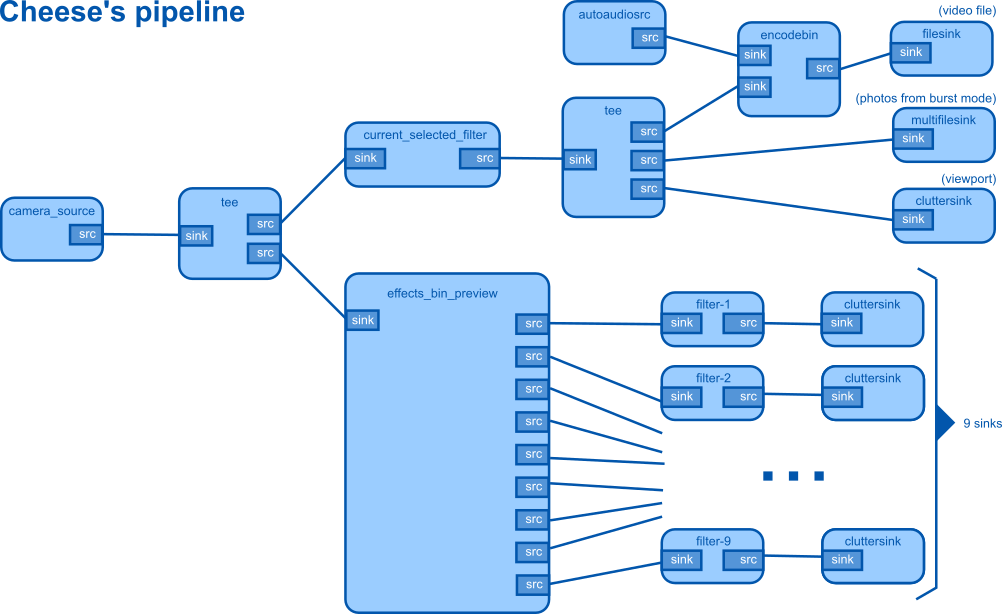
\includegraphics[angle=90,width=0.8\textwidth]{../images/cheese-pipeline.png}\par
  \caption{Simplificación del \textit{pipeline} de Cheese. Imagen inspirada a
  				 partir de la generación de un diagrama en Graphviz con GStreamer en
  				 modo DEBUG}
  \caption*{Fuente: Autoría propia}
\end{figure}

\section{OpenCV}
Es una librería para visión artificial en tiempo real. Es software de código
abierto siendo licenciada bajo la licencia BSD. Fue inicialmente desarrollado
por Intel Inc \cite{openCVAbout}. Está escrita en C y C++ con bindings para
otros lenguajes de programación como Python y Java. Entre los distintos
algoritmos que implementa OpenCV se encuentra la detección de objetos usando
el algoritmo propuesto por Paul Viola y Michael Jones en “Rapid Object Detection
using a Boosted Cascade of Simple Features” y el algoritmo para la estimación de
 variables llamado filtro de Kalman. \cite{openCVAbout}.
\section{dlib}
Es una librería que implementa una amplia cantidad de algoritmos en aprendizaje
de máquina. Es software de código abierto licenciado bajo la
licencia Boost License y escrita en C++ \cite{dlib}\cite{dlibLicense}. Entre
los distintos algoritmos que implementa se encuentra el propuesto por Navneet
Dalal y Bill Triggs en “Histograms of Oriented Gradients for Human Detection”
\cite{dlibHOG} y la detección del “landmark” del rostro con el algoritmo
propuesto por Vahid Kazemi y Josephine Sullivan en “One Millisecond
Face Alignment with an Ensemble of Regression Trees” \cite{dlib1ms}.

\chapter{Estado del Arte}
\section{Revisión y discusión}

En esta sección, se analiza qué librerías se debería escoger no solo por la
disponibilidad de algoritmos útiles para realizar el seguimiento de rostros sino
que sus licencias deben ser compatibles con Cheese. El método a seguir en este
análisis es el de la revisión sistemática. En este método se plantea preguntas
que son de la duda del autor para posteriormente analizarlas a detalle.\\

\subsubsection{Palabras clave}
A continuación, se muestra una lista de algunas palabras clave que fueron
introducidos en los buscadores de Google y Github con el fin de resolver dudas.

En relación a librerías a usar:

\begin{itemize}
	\item face tracking open source free software library
	\item dlib users
	\item opencv users
	\item face tracking dlib
	\item face tracking open cv
	\item 4dface
	\item 3d face tracking
	\item Landmark
\end{itemize}

En relación a las licencias:
\begin{itemize}
	\item GPLv2 compatibility Boost license
	\item GPLv2 compatibility MIT license
	\item GPLv2 compatibility BSD license
	\item GPLv2 compatibility Apache license
\end{itemize}

\subsubsection{Preguntas a resolver}

\noindent
\textbf{P1}: ¿Qué librería se debería usar siendo esta la que tenga mayor soporte
por la comunidad de software libre de tal manera que se pueda esperar que
Cheese dure en el largo plazo sin revertir los cambios debido a problemas en
las dependencias?\\
\textbf{P2}: ¿Qué librería que sea compatible con GPLv2 usar?\\
\textbf{P3}: ¿Qué librería se debe usar?

\subsection{Librerías a considerar según su soporte para realizar seguimiento
						de rostros}
Según la búsqueda realizada dio como posibles opciones a usar \textit{4dface},
\textit{OpenCV}, \textit{dlib} y \textit{FaceX}. Estas librerías están escritas
tanto en C++ como en C, lo cual significa que pueden ser empleadas sobre
GStreamer cuya implementación de plugins está soportada especialmente en C y C++
por la comunidad.
\textit{4dface} es una librería escrita en C++ que soporta directamente el
seguimiento debe rostros en tiempo real y la reconstrucción de la forma de un
rostro a partir de imágenes en tiempo real (un aproximado de 5fps); esta librería
está desarrollada para integrarse con OpenCV \cite{4dface}. \textit{OpenCV}, a
diferencia de \textit{4dface} no soporta directamente el seguimiento de rostros
en tiempo real ni tampoco la detección del landmark. No obstante, está soportada
la detección de rostros, y aunque no es suficiente por sí misma, debido a lo
expuesto en el capítulo de la Problemática, se puede combinar con el uso del
algoritmo del filtro de Kalman o con Camshift, los cuales están implementados.
En una situación parecida se encuentra \textit{dlib} que tampoco está
especializado en el rastreo de rostros, pero soporta la detección de
\textit{landmarks}. Finalmente, \textit{FaceX} está especializado en la
detección de landmarks \cite{FaceX}.

\subsection{Librerías de detección y/o segumiento de rostros según su
            popularidad}
Es importante buscar una librería ampliamente soportada por la comunidad de
software libre que pueda ser útil para implementar el algoritmo de seguimiento
de rostros y landmark a partir de videos (como capturas de la cámara web) en
tiempo real.

Para ello solo serán consideradas librerías que aparecieron en las primeras
páginas de las búsquedas, pues esto da un indicio de que son las más populares.
Además se descartarán todas aquellas librerías cuya última actualización haya
sido mayor a 2 años; por ejemplo, en caso de usar Git para el control de
versiones, cuyo último commit sea mayor a 2 años. Además, en caso de usar Git,
solo se considerarán librerías con más ``forks'', más ``watch'' y más ``stars''
(métricas de Github). En la búsqueda realizada se encontró que las siguientes
librerías podrían ser útiles para resolver el problema.

\begin{center}
	\begin{table}[h]
      \begin{tabular}{| l | l | l | l | l |}
      \hline
      Programa & último commit & forks & stars & watch \\ \hline
      OpenCV & 09-09-2017 & 13494 & 18075 & 1693 \\ \hline
      4dface & 02-12-2016 & 133 & 268 & 44 \\ \hline
      dlib & 10-09-2017 & 936 & 2701 & 262 \\ \hline
      FaceX & 15-11-2015 & 86 & 95 & 18 \\ \hline
      \end{tabular}
      \caption{Tabla construida en base a las métricas de los proyectos en Github
               al 10-09-2017.}
      \caption*{Fuente: Repositorios de los proyectos en \textit{git}}
	\end{table}
\end{center}

Se puede observar que las más populares son OpenCV y dlib. OpenCV según su
página web cuenta con más 47 mil usuarios y un número de descargas que exceden
los 14 millones \cite{OpenCV}. Mientras dlib en su página web también asegura
tener varios usados además de estar citado en distintas investigaciones
académicas \cite{dlibUsers}.

\subsection{Librerías de detección y/o segumiento de rostros según su
            compatibilidad con GPLv2}
Saber que licencia es compatible con GPLv2 es importante porque si no fuera así,
sería complicado que el cambio sea aceptado en Cheese o que sea aplicado a un
fork de este. De hecho, si no se realiza esta tarea desde el principio, y se
optara por error por una dependencia con licencia incompatible, el trabajo
realizado podría resultar vano. GPLv2 es una licencia de software libre, pero
tiene ciertas limitaciones respecto a GPLv3.

\begin{center}
	\begin{table}[h]
      \begin{tabular}{| l | l | l |}
      \hline
      Programa & Licencia & ¿Compatible con GPLv2? \\ \hline
      OpenCV & BSD License & Sí \\ \hline
      4dface & Apache License 2.0 & No \\ \hline
      dlib & Boost Software License 1.0 & Sí \\ \hline
      FaceX & MIT License & Sí \\ \hline
      FaceX-train & GPLv3 & Sí \\ \hline
      \end{tabular}
      \caption{Tabla de comparación de programas según su compatibilidad con GPLv2.}
      \caption*{Fuente: Repositorios de los proyectos en \textit{git}
                \cite{openCVLicense}\cite{dlibLicense2}\cite{faceXLicense}
                \cite{4dfaceLicense} y para la compatibilidad con GPLv2 la web de
                la FSF \cite{GPLv2Compatibility}}
	\end{table}
\end{center}


\section{Conclusiones}
Si bien \textit{4dface} podía ser una buena alternativa por sus características,
se descarta la posibilidad de su uso esencialmente debido a ser incompatible
con la licencia de Cheese. \textit{FaceX} también se descarta porque no hay
indicios para pensar que su desarrollo continuará en los siguientes años. Tanto
\textit{OpenCV} como \textit{dlib} parecen ser la mejor opción no solo porque
son compatibles con la licencia de Cheese, sino también porque implementan
algoritmos que son útiles para el seguimiento de objetos (en este caso rostros)
en tiempo real y detección de landmark. La combinación de ambos representa una
alternativa factible para solucionar el problema.

\chapter{Filtro de detección, rastreamiento y detección de puntos faciales de
múltiples rostros: \textit{gstcheesefacetrack}}
Este capítulo consta de tres partes específicas. En la primera sección, se
detalla paso a paso y explica el algoritmo implementado para el rastreamiento de
múltiples rostros y detección de puntos faciales cuya implementación como filtro
para \textit{GStreamer} se llamó \textit{gstcheesefacetrack}. En la siguiente
sección, se explica cómo usar el filtro con algunos ejemplos incluidos. Y
finalmente, en la última sección, se mostrarán algunas métricas como
\textit{f1-score}, \textit{accuracy} y \textit{recall}.

\section{Algoritmo de detección y rastreamiento de múltiples rostros y
de detección puntos faciales}

\subsection{Introducción}
El algoritmo desarrollado consiste en ciclos, en los cuales por cada ciclo en
el primer cuadro se detectan los rostros y en los siguientes cuadros se realiza
rastrea a los rostros. La detección de rostros suele ser un proceso costoso
comparado con el rastreo, es por ello que mientras más largo sea el tiempo en el
cual se rastrea los rostros habrá menos latencia. Sin embargo, a veces puede que
nuevas personas entren a la escena capturada por la cámara web o que algunas
personas salgan de esta. Además puede suceder que el rastreador pierda su objetivo o
el resultado de este sea poco probable. Es por esta razón que es necesario cada
cierto tiempo detectar rostros. La detección de rostros que solo se raliza una
vez cada ciclo es aprovechada para verificar si rostros de personas entraron o
salieron de la escena. Además esta fase de detección es una oportunidad para
verificar si el rastreador está dando resultados probablemente correctos o no.
Si el rastreador dice que hay un rostro donde en verdad según el detector no
existe ninguno, esto se corrige en esta fase. En esta fase de detección, además,
se reasignan (o reordenan) los rostros de tal manera que cada rostro detectado
preserve su identidad. Además de ello, a veces puede suceder que el rastreador
pierda su objetivo (el rostro rastreado). Este caso es un caso de urgencia y
excepción al ciclo explicado inicialmente, y se entrará en una fase de
detección.

\begin{figure}[!h]
  \centering
    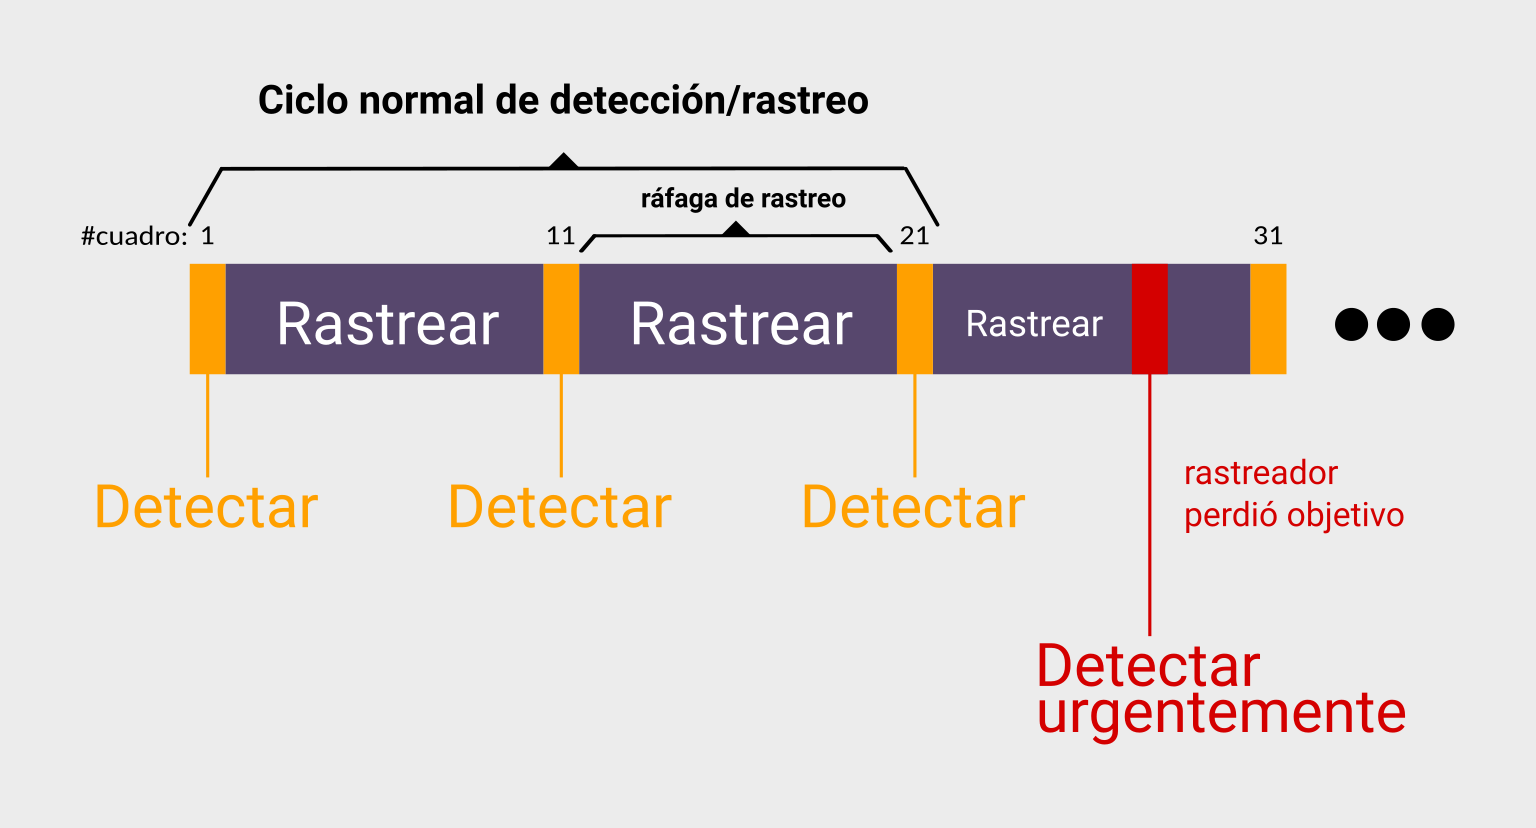
\includegraphics[width=1.0\textwidth]{../images/diagrama-rafagas-cheesefacetrack.png}\par
  \caption{Diagrama de ciclo de ciclo de detección y rastreo realizado por
           el algoritmo}
    \label{fig:diagrama-rafagas-cheesefacetrack}
  \caption*{Fuente: Autoría propia}
\end{figure}

\subsection{¿Cómo se almacena la información de los rostros?}
Cada rostro es único. Las tablas hash permiten tener llaves únicas (que no se
repiten) y además tienen tiempo de acceso $O(1)$, por tanto guardar información
de cada rostro en una tabla hash ha resultado conveniente para este algoritmo.
La llave de la tabla hash es un número identificador ($id$) y el valor
relacionado a esta llave es una estructura que contiene información específica
del rostro.\\
La estructura definida contiene la información del rectángulo ($rectángulo$) y
puntos faciales ($landmark$) que delimita el rostro en el último cuadro en el
cual este fue detectado o rastreado. Cada estructura además tiene un rastreador
($rastreador$) el cual es definido a gusto del usuario y puede ser Median Flow,
MIL, KCF, TLD o Boosting de los cuales se recomienda Median Flow. Antes de crear
un rastreador, ningún rastreador ha sido asignado al rostro (estado
$NO\_ASIGNADO$), luego al asignarse un rastreador ($rastreador$) este pasa al
estado ($NO\_INICIALIZADO$): ambos estados mencionados son solo de paso. Cuando
se inicializa el rastreador se pasa al estado de inicializado ($INICIALIZADO$)
y cuando se empieza el proceso de rastreo este pasa a estado de rastreando
($RASTREANDO$). Finalmente, se guarda el último número de cuadro en el cual el
rostro fue detectado.

\begin{algorithm}
\floatname{algorithm}{Estructura}
\caption{Estructura que contiene la información de la \textit{\textbf{identidad}}
         de un rostro}
\label{euclid}
\begin{algorithmic}
\State \textbf{estructura} RostroT $\{$
\Indent
  \State $rectángulo$, Rectángulo que delimita el rostro de la cara.
  \State $landmark$, Arreglo de puntos faciales. Inicialmente vacía.
  \State $rastreador$, El rastreador qué puede ser Median Flow, MIL,
                        KCF, TLD o Boosting, según sea especificado como
                       parámetro.
  \State $estadoRastreador$, El estado del rastreador el cuál puede ser
                            $NO\_ASIGNADO$, $NO\_INICIALIZADO$, $INICIALIZADO$,
                            o $RASTREANDO$. Inicialmente $NO\_INICIALIZADO$.
  \State $ultimoCuadroDetectado$, el número de cuadro en el cual el rostro fue
                                 detectado o rastreado por última vez.
\EndIndent
\State  $\}$
\end{algorithmic}
\end{algorithm}

\subsection{Explicación detallada del algoritmo}
El algoritmo propuesto cuyo (pseudocódigo principal puede verse en el cuadro
titulado algoritmo~\ref{alg:tracking}) ejecuta un procedimiento cíclicamente
para cada cuadro de video capturado (en este caso por la cámara web). Este
procedimiento inicia escalando la imagen por un factor de escala
($factor\_escala$), la razón de ello es para agilizar la detección de rostros.
Una variable global $ROSTROS\_TABLA$ la cual es una tabla hash tal como se
describió en la sesión anterior está inicialmente vacía, pues aun no se ha
procesado ningún rostro, por ello las
líneas~\ref{lst:line:initBefDetect}-\ref{lst:line:endBefDetect} serán
explicadas más adelante. Las siguientes subsecciones explican a detalle cada
parte del algoritmo.\\

\begin{algorithm}
  \caption{Algoritmo de rastreamiento y detección de puntos faciales}
  \label{alg:tracking}
  \textbf{Global: }$ROSTROS\_TABLA$, tabla hash \textbf{inicialmente vacía}
      (llave: \textit{entero}, valor: rectángulo delimitador y \textit{landmark})\\
  \textbf{Global: }$\acute{U}LTIMO\_ID$, el siguiente identificador a asignar. Valor inicial: $0$\\
  \textbf{Global: }$TIPO\_RASTREADOR$, el tipo de rastreador a usar que puede
                                       ser Median Flow, MIL, KCF, TLD o
                                       Boosting, según sea especificado como
                                        parámetro.\\
  \textbf{Global: }$N$, el número de cuadro actual. Valor inicial: $1$\\
  \textbf{Parámetro: }$factor\_escala \in [0, 1]$\\
  \textbf{Parámetro: }$factor\_distancia \in [0, 1]$\\
  \textbf{Parámetro: }$brecha\_detecci\acute on \in \mathbb{N}$\\
  \textbf{Parámetro: }$borrado\_threshold \in \mathbb{N}$\\
  \algorithmicrequire{$I$, una imagen de dimensiones $ancho \times largo$}\\
  \begin{algorithmic}[1]
    \Procedure{ProcesarCuadro}{$I$}

      \State $I_{s}\leftarrow I \times factor\_escala$ \Comment{Escalar imagen.}
      \State IdsRostrosPerdidos$\leftarrow []$ \label{lst:line:A}\Comment{Lista de \textit{ids} de
                                                        rostros cuyo rastreador
                                                        perdió el objetivo.}
      \State IdsRostrosNoCreados$\gets []$ \Comment{Lista de \textit{ids} de
                                                        rostros no creados en el
                                                        cuadro actual.}

      \State \Call{IntentarBorrarRostros}{}
      \label{lst:line:initBefDetect}
      \For{(id, rostro) \textbf{en} $ROSTROS\_TABLA$}
      \label{lst:line:faseDetec}
        \State $\acute{e}xito \gets$ rostro.\Call{rastrear}{$I_{s}$}
        \label{lst:line:rastrear}
        \If{$\acute{e}xito$}
          \State rostro.ultimoCuadroDetectado $\gets N$
          \label{lst:line:rastrearActualizarUltimoFrame}
        \Else
          \State IdsRostrosPerdidos.\Call{agregar}{id} \label{lst:line:objetivoPerdido}
          \label{lst:line:registrarPerdidos}
        \EndIf
          \State IdsRostrosNoCreados.\Call{agregar}{id}
      \EndFor \label{lst:line:B}
      \label{lst:line:endBefDetect}

      \State enFaseDeDeteccion$\gets$ $N$ \textbf{mod} $brecha\_detecci\acute on$ $= 1$ \label{lst:line:C}

      \If{enFaseDeDeteccion \textbf{o} \Call{longitud}{IdsRostrosPerdidos} $> 0$} \label{lst:line:inicioFaseDetect}
        \State detsRz $\gets$ detectarRostros($I_{s}$) \Comment{Lista de rectángulos.} \label{lst:line:deteccion}
        \If{\Call{longitud}{$ROSTROS\_TABLA$} $= 0$}
          \State \Call{crearYAgregarRostros}{$ROSTROS\_TABLA$, $I_{s}$, detsRz};
          \label{lst:line:crearYAgregarRostrosA}
        \EndIf

        \If{\Call{longitud}{IdsRostrosNoCreados} $> 0$ \textbf{y} \Call{longitud}{detsRz} $> 0$}
          \label{lst:line:checkIfHungarian}
          \State centroidesRostrosDetectados $\gets$
              \lbrack\Call{centroide}{$r$} \textbf{para} $r$ \textbf{en} detsRz\rbrack
          \label{lst:line:costMatrixInit}
          \State centroidesRostrosNoCreados $\gets$
              \lbrack \Call{centroide}{$r$} \textbf{para} $r$ \textbf{en} $ROSTROS\_TABLA$[IdsRostrosNoCreados].rectángulos\rbrack
          \State MatrizDeCostos$\leftarrow$\Call{inicializarMatrizDeCostos}{centroidesRostrosDetectados, centroidesRostrosNoCreados}
          \label{lst:line:costMatrixEnd}
          \State asignaciones$\gets$\Call{métodoHúngaro}{MatrizDeCostos}
          \Comment{\textcolor{red}{Continúa...}}
      \algstore{myalg}
  \end{algorithmic}
\end{algorithm}

\clearpage

\begin{algorithm}
  \ContinuedFloat
  \caption{Algoritmo de rastreamiento y detección de puntos faciales (continación)}
  \begin{algorithmic}
      \algrestore{myalg}
          \For{$i\gets0$ \textbf{hasta} \Call{longitud}{centroidesRostrosDetectados}}
          \label{lst:line:iterRostros}
            \State asignado$\leftarrow$asignaciones[$i$]$\neq-1$
            \State crearRostro$\leftarrow$\textit{verdadero}

            \If{asignado}
            \label{lst:line:asignadoInit}
              \State id$\gets$IdsRostrosNoCreados\lbrack asignaciones\lbrack$i$\rbrack\rbrack
              \State rostro$\gets ROSTROS\_TABLA[$id$]$
              \State crearRostro$\gets$\textit{falso}
              \State $c1\gets$\Call{centroide}{centroidesRostrosDetectados$[i]$}
              \State $c2\gets$\Call{centroide}{rostro.rectángulo}
              \State distancia$\gets$\Call{distanciaEuclidiana}{$c1$,$c2$}
              \State maxDistancia$\gets$$factor\_distancia \times $detsRz.ancho
              \If{distancia $\geq$ maxDistancia}
                \State rostro.rastreador.\Call{liberar}{}()
              \EndIf
            \EndIf
            \label{lst:line:asignadoFin}
            \If{crearRostro}
              \State \Call{crearYAgregarRostros}{$ROSTROS\_TABLA$, $I_{s}$, [detsRz[$i$]]}
            \Else
              \State id$\gets$IdsRostrosNoCreados\lbrack asignaciones\lbrack$i$\rbrack\rbrack
              \label{lst:line:initResetFaces}
              \State rostro$\gets ROSTROS\_TABLA[$id$]$
              \If{rostro.estadoRastreador $= NO\_ASIGNADO$}
                \State rostro.rectángulo$\gets$detsRz[$i$]
                \State rostro.\Call{crearRastreador}{$tracker$}
                \State rostro.\Call{inicializarRastreador}{$I_{s}$}
                \State rostro.ultimoCuadroDetectado $\gets N$
              \EndIf
              \label{lst:line:endResetFaces}
            \EndIf
          \EndFor
        \EndIf
      \EndIf \label{lst:line:finFaseDetect}
      \For{(id, rostro) \textbf{en} $ROSTROS\_TABLA$}
        \State mostrarRostro$\gets$ rostro.ultimoCuadroDetectado $= N$
        \If{$mostrarRostro$}
          \If{rostro.estadoRastreador $= INICIALIZADO$}
            \State rostro.landmark $\gets$ \Call{detectarPuntosFaciales}{$I_{s}$}
            \label{lst:line:estimarLandmark}
          \EndIf
          \State \Call{MostrarRostro}{rostro}
          \label{lst:line:mostrarRostros}
        \EndIf
      \EndFor
      \State $N\gets N + 1$
    \EndProcedure
  \end{algorithmic}
\end{algorithm}

\subsubsection{Fase de detección}
Se empieza por analizar si el número de cuadro actual corresponde a una fase de
detección normal (algoritmo~\ref{alg:tracking}, línea~\ref{lst:line:C}).
La fase de detección se da en el primer cuadro
y cada cierta cantidad de cuadros $brecha\_detecci\acute on \in \mathbb{N}$.
También existe un caso en el cual se puede entrar a la fase de detección que
sucede si alguno de los rastreadores asignado a un rostro perdió su objetivo
(algoritmo~\ref{alg:tracking}, línea~\ref{lst:line:objetivoPerdido}).\\
La fase de detección
(algoritmo~\ref{alg:tracking}, líneas~\ref{lst:line:inicioFaseDetect}-\ref{lst:line:finFaseDetect})
inicia con la detección de rostros
(algoritmo~\ref{alg:tracking}, líneas~\ref{lst:line:deteccion}) usando un
detector de objetos siguiendo el método de histograma de gradientes
(\textit{HOG}). De no haber rostros previamente registrados en la tabla hash
$ROSTROS\_TABLA$, se procede a crear una entrada en esta tabla para cada
rostro detectado (algoritmo~\ref{alg:tracking},
línea~\ref{lst:line:crearYAgregarRostrosA}, con más detalles en el apartado
\ref{sssec:create}). Para el cuadro actual, de no haber habido rostros
previamente a los detectados (o creados) durante la fase de detección y de haber
nuevos rostros detectados en el cuadro actual (algoritmo~\ref{alg:tracking},
líneas~\ref{lst:line:checkIfHungarian}), se procede a construir el problema de
asignación.\\
El problema de asignación planteado se pregunta: ``¿Qué rostro
no creado antes de la fase de detección (en el cuadro actual) debe asignarse o
está más cerca (y por tanto más probable) al rostro actualmente detectado'',
debido a que en esta fase los rostros se desordenan. A continuación se detalla
un ejemplo sencillo de este problema.\\

\begin{figure}[!h]
  \centering
    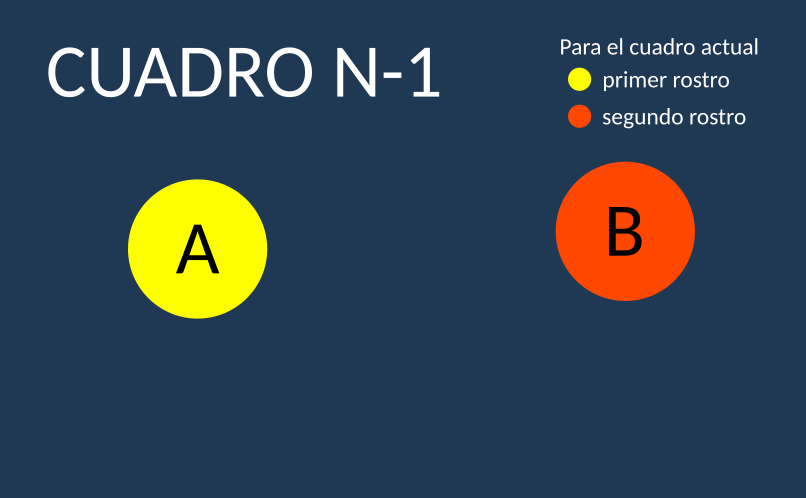
\includegraphics[width=0.7\textwidth]{../images/hungarian-example-1.png}\par
  \caption{Representación de la disposición de los rostros rastreados un cuadro
           antes de la fase de detección. Los círculos amarillo y rojo
           representan cada uno un rostro, mientras las letras $A$ y $B$
           representan los identificadores de cada rostro}
    \label{fig:hungarian-example-1}
  \caption*{Fuente: Autoría propia}
\end{figure}

\begin{figure}[!h]
  \centering
    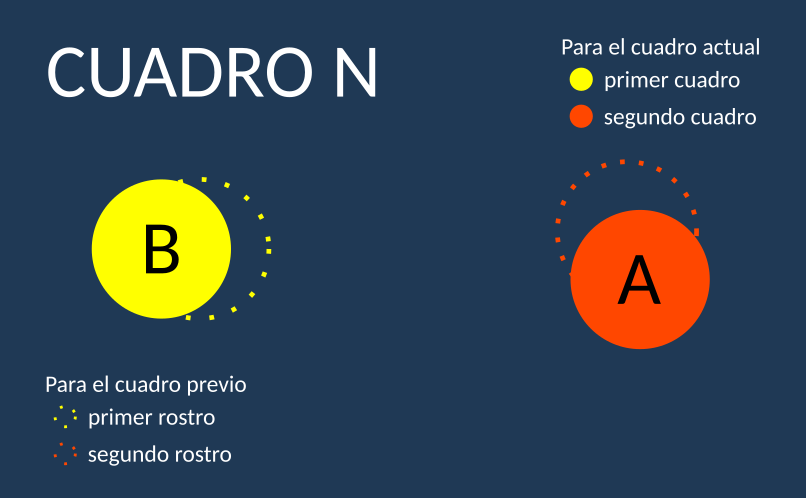
\includegraphics[width=0.7\textwidth]{../images/hungarian-example-2.png}\par
  \caption{Representación de lo que sucede durante la fase de detección. Las
           líneas punteadas representan las posiciones anteriores de los
           rostros. Se observa que el detector de rostros intercambió los
           identificadores $A$ y $B$ en el orden $B$ y $A$. Evidentemente,
           el orden debería ser $A$ y $B$}
    \label{fig:hungarian-example-2}
  \caption*{Fuente: Autoría propia}
\end{figure}

En la figura \ref{fig:hungarian-example-1},
se observa la representación de los rostros que fueron rastreados un cuadro
antes de la fase de detección (izquierda: A, derecha: B). Luego, en la figura
\ref{fig:hungarian-example-2}, se representa la fase
de detección, donde los rostros se han movido ligeramente pero según el
detector, las etiquetas se han cambiado (izquierda: B, derecha: A). Lo esperado,
sería seguir manteniendo el orden inicial de las etiquetas. Es poco probable que
de un cuadro a otro un rostro se haya movido mucho, por lo tanto debe estar muy
cercano a su posición previa. En la figura \ref{fig:hungarian-example-3}, se
procede a medir las combinaciones de distancias con el propósito de encontrar
cuáles son los rostros más cercanos a los rostros detectados actualmente. Se
observa a simple vista, que para el rostro más cercano al rostro detectado de la
izquierda (en amarillo) en el cuadro $N$ la distancia más cercana es $d1$ y que
para el rostro detectado de la derecha (en rojo) es $d2$. Finalmente, en la
figura \ref{fig:hungarian-example-4} se ve que las etiquetas $A$ y $B$ son
reasignadas correctamente. El problema de asignación planteado anteriormente, es
fácil de resolver en el ejemplo de la figura. Sin embargo, este se complica
cuando hay más rostros y estos están muy cerca, es por ello que debe usarse un
método más genérico.\\

\begin{figure}[!h]
  \centering
    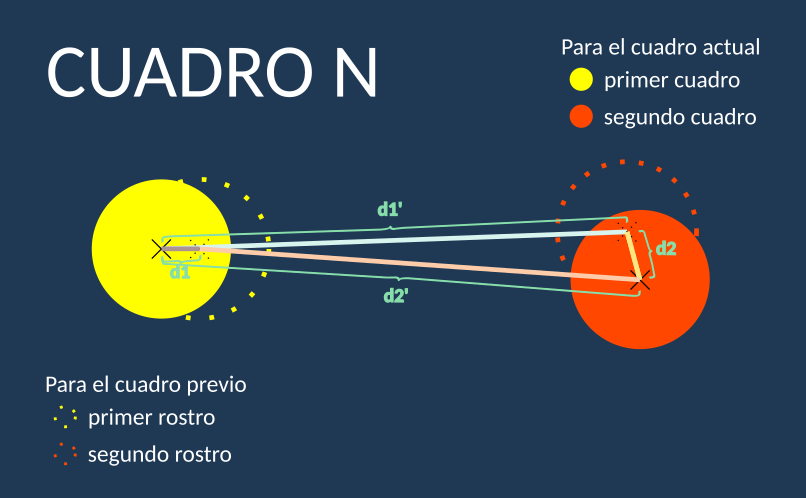
\includegraphics[width=0.7\textwidth]{../images/hungarian-example-3.png}\par
  \caption{Cálculo de las distancias entre los rostros no detectados en el
           cuadro anterior a la fase de detección y los rostros detectados
           durante la fase de detección. Se observa que $d1$ y $d2$ son las
           distancias menores.}
    \label{fig:hungarian-example-3}
  \caption*{Fuente: Autoría propia}
\end{figure}

\begin{figure}[!h]
  \centering
    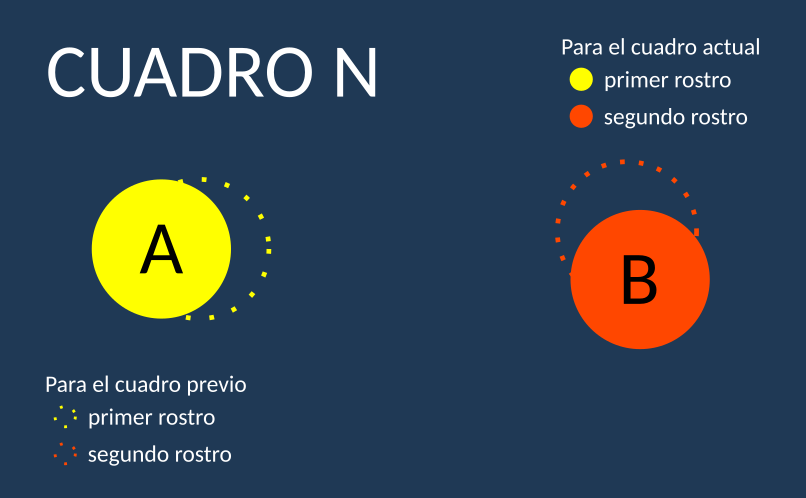
\includegraphics[width=0.7\textwidth]{../images/hungarian-example-4.png}\par
  \caption{Estado final de las etiquetas $A$ y $B$ tras resolver el problema de
           asignación.}
    \label{fig:hungarian-example-4}
  \caption*{Fuente: Autoría propia}
\end{figure}

El problema de asiganación planteado se resuelve mediante el método húngaro. Se
define una matriz de costos ($MatrizDeCostos$) cuyas filas corresponde a ``la
cantidad de rostros no creados en el cuadro actual antes de la fase de
detección'' y cuyas columnas corresponde a la cantidad de ``rostros detectados
en el cuadro actual''. Cada elemento de la matriz ($MatrizDeCostos_{i,j}$)
corresponde a la distancias euclidianas entre el centroide del
``rostro no creados antes de entrar a la fase de detección'' en la posición
$i$ respecto al centroide del ``rostro detectado en el cuadro actual'' en
la posición $j$ (algoritmo~\ref{alg:tracking},
líneas~\ref{lst:line:costMatrixInit}-\ref{lst:line:costMatrixEnd}).\\

Debido a que la matriz de costos puede no ser cuadrada, habrá algunos rostros
que no se serán asignados. Otro problema es que el resultado de asignar ``un
rostro no detectado antes de la fase de detección'' a uno ``detectado en el
cuadro actual'' puede estar muy lejos por diversas razones (por ejemplo, el
detector detectó un rostro cuando anteriormente se registraba dos rostros). Para
verificar si sucede algunos de estos problemas se itera sobre cada rostro
detectado (algoritmo~\ref{alg:tracking}, líneas~\ref{lst:line:iterRostros}). Si
el rostro detectado fue asignado, se verifica que esté suficientemente cerca (es
decir que la distancia al rostro asignado no exceda un límite o
\textit{threshold} equivalente a $factor\_distancia$ veces el ancho del
rectángulo delimitador del rostro detectado). De no estar suficientemente cerca,
el rastreador relacionado a este rostro se libera y su estructura pasa a estado
no disponible ($NO\_ASIGNADO$). Ver algoritmo~\ref{alg:tracking},
líneas~\ref{lst:line:asignadoInit}-\ref{lst:line:asignadoFin}. De no haber sido
asignado el rostro detectado, se procede a crear una entrada en esta tabla para
cada rostro detectado (algoritmo~\ref{alg:tracking},
línea~\ref{lst:line:crearYAgregarRostrosA}, con más detalles en el apartado
\ref{sssec:create}), ya que puede tratarse de un nuevo rostro que ingresó a la
escena. En caso contrario (algoritmo~\ref{alg:tracking},
línea~\ref{lst:line:initResetFaces}-\ref{lst:line:endResetFaces}), se reinicia
un rastreador para la estructura correspondiente y se actualiza el último cuadro
en el cual el rostro fue detectado en la estructura
($RostroT.ultimoCuadroDetectado$).\\

\subsubsection{Borrado o limpieza de rostros no detectados recientemente}
En la línea~\ref{lst:line:initBefDetect}, se llama al procedimiento
$IntentarBorrarRostros$. Aquí se borran los rostros que no fueron detectados o
rastreados hace $borrado\_threshold$ cuadros de la tabla hash de rostros. Esta
limpieza se debe a que a medida que pasa el tiempo es posible que un rostro se
haya movido mucho o incluso que el rostro haya salido de la escena. El
identificador para este rostro será simplemente desechado y nunca más podrá
volver a usarse. Ver algoritmo~\ref{alg:delete} para más detalles.\\

\subsubsection{Fase de rastreo}
La mayor parte del tiempo se realiza rastreo de rostros. Si bien existe una
amplia variedad de rastreadores a elegir como Median Flow, MIL, KCF, TLD,
Boosting, entre otros, se recomienda Median Flow, puesto que es capaz de
estimar la escala del objetivo (por ejemplo, si el rostro se aleja o se acerca).
Durante cada cuadro en la fase de detección que son los cuadros restantes
luego de la fase detección (durante $brecha\_detecci\acute on - 1$ cuadros), se
intenta predecir (algoritmo~\ref{alg:tracking}, línea~\ref{lst:line:rastrear})
la posición actual de cada rostro en la tabla hash de estructuras
($ROSTRO\_TABLA$). De predecir la posición del rostro exitosamente, se modifica
la estructura del rostro respectivo actualizando el último cuadro detectado al
actual (algoritmo~\ref{alg:tracking},
línea \ref{lst:line:rastrearActualizarUltimoFrame}). De lo contrario,
si el rastreador perdió su objetivo, se agrega el identificador del rostro a una
lista para ser usada en la fase de detección (algoritmo~\ref{alg:tracking},
línea \ref{lst:line:registrarPerdidos}).\\


\subsubsection{Creación y agregado rostros a la tabla hash} \label{sssec:create}
Este procedimiento se encarga de crear para cada rectángulo delimitadir las
estructuras de rostros y asignarles el siguiente identificador disponible
(algoritmo~\ref{alg:create},
línea \ref{lst:line:createRastrearActualizarUltimoFrame}). Para cada nueva
estructura de rostro creada se le asigna el rectángulo delimitador y se crea e
inicializa un rastreador para cada estructura (algoritmo~\ref{alg:create},
línea \ref{lst:line:createBeginNewStruct}-\ref{lst:line:createEndNewStruct}).\\

\begin{algorithm}
  \caption{Procedimiento que crea nuevos rostros con rastreadores inicializados
           y los inserta en tabla hash}
  \label{alg:create}
  \textbf{Global: }$ROSTROS\_TABLA$, tabla hash \textbf{inicialmente vacía}
      (llave: \textit{entero}, valor: rectángulo delimitador y \textit{landmark})\\
  \textbf{Global: }$TIPO\_RASTREADOR$, el tipo de rastreador a usar que puede
                                       ser Median Flow, MIL, KCF, TLD o
                                       Boosting, según sea especificado como
                                       parámetro.\\
  \textbf{Global: }$\acute{U}LTIMO\_ID$, el siguiente identificador a asignar. Valor inicial: $0$\\
  \textbf{Global: }$N$, el número de cuadro actual. Valor inicial: $1$\\
  \begin{algorithmic}[1]
    \Procedure{crearYAgregarRostros}{$ROSTROS\_TABLA,I,rect\acute{á}ngulos$}
      \For{$rectángulo$ \textbf{en} $rect\acute{á}ngulos$}
        \State $\acute{U}LTIMO\_ID\gets \acute{U}LTIMO\_ID + 1$
        \label{lst:line:createRastrearActualizarUltimoFrame}
        \State rostro$\gets$ \textbf{instanciar} $RostroT$
        \label{lst:line:createBeginNewStruct}
        \State rostro.ultimoCuadroDetectado$\gets N$
        \State rostro.rectángulo $\gets rectángulo$
        \State $ROSTRO[\acute{U}LTIMO\_ID]\gets$rostro
        \State $ROSTRO[\acute{U}LTIMO\_ID].$\Call{crearRastreador}{$TIPO\_RASTREADOR$}
        \State $ROSTRO[\acute{U}LTIMO\_ID].$\Call{inicializarRastreador}{$I$}
        \label{lst:line:createEndNewStruct}
      \EndFor
    \EndProcedure
  \end{algorithmic}
\end{algorithm}

\subsubsection{Detección de puntos faciales y mostrado de rostros} \label{sssec:landmark}
Una vez terminada la fase de detección, con la tabla hash $ROSTROS\_TABLA$
(probablemente) llena, para cada rostro se estima los puntos faciales
(\textit{landmarks} ignorando los rostros cuyo último cuadro de detección
($ultimoCuadroDetectado$) fue anterior a $N$. Para ello, tomando el rectángulo
delimitador de cada rostro se aplica un algoritmo de alineación de
rostros con un conjunto de árboles de regresión (algoritmo~\ref{alg:create},
línea \ref{lst:line:estimarLandmark}) que permite detectar los
\textit{landmarks} de cada rostro en milisegundos. Finalmente, todos estos
rostros son considerados rostros presentes en el cuadro actual y son objeto de
procesamiento (algoritmo~\ref{alg:create}, línea \ref{lst:line:mostrarRostros};
por ejemplo, para dibujar los rectángulos delimitadores y los puntos faciales).

\begin{algorithm}
  \caption{Borrado de información de rostros que no han sido detectados o
      rastreados durante un tiempo considerable}
  \label{alg:delete}
  \textbf{Global: }$ROSTROS\_TABLA$, tabla hash \textbf{inicialmente vacía}
      (llave: \textit{entero}, valor: rectángulo delimitador y \textit{landmark})\\
  \textbf{Global: }$N$, el número de cuadro actual. Valor inicial: $1$\\
  \textbf{Parámetro: }$borrado\_threshold \in \mathbb{N}$\\
  \begin{algorithmic}[1]
    \Procedure{IntentarBorrarRostros}{}
      \For{(id, rostro) \textbf{en} $ROSTROS\_TABLA$}
        \State $\Delta\gets N - $rostro.ultimoCuadroDetectado
        \If{$\Delta > borrado\_threshold$}
          \State \Call{borrar}{$ROSTROS[id]$}
        \EndIf
      \EndFor
    \EndProcedure
  \end{algorithmic}
\end{algorithm}

\subsection{Explicación del nombre \textit{gstcheesefacetrack}}
Al filtro desarrollado se le ha asignado el nombre de
\textit{gstcheesefacetrack} y \textbf{en adelante se hará referencia a este
filtro por este nombre}. La asignación del nombre se explica a continuación:
como la mayoría de elementos de \textit{GStreamer} tiene en su nombre el prefijo
\textit{gst} y además se le pone el prefijo \textit{cheese} debido al programa
al cual se aplicará. Luego, lleva el término \textit{face} debido a que está
ubicado en el directorio \textit{gst-plugins-cheese/gst/face} lugar donde se
ubica filtros que usan datos de lo rostros. Finalmente, \textit{track} se debe
a que este algoritmo se encarga principalmente de rastrear rostros.

\section{Diseño y \textit{capabilities}}
El filtro \textit{gstcheesefacetrack} hereda del filtro
\textit{gstopencvvideofilter}. Consecuentemente, los \textit{pad templates} son
los mismos que los que usa el filtro \textit{gstopencvvideofilter}, y por ende,
las \textit{capabilities} (formatos de video, \textit{fps}, dimensiones, entre
otras propiedades que se definen para ser aceptadas) son las mismas que las de
\textit{gstopencvvideofilter}.\\

\section{Propiedades}
Las propiedades del filtro son las siguientes:
\begin{center}
  \begin{longtable}{| p{.2\textwidth} | p{.2\textwidth} | p{.6\textwidth} |}
  \hline

  % Cabecera
  \textbf{Propiedad} &
  \textbf{Tipo} &
  \textbf{Descriptión de la propiedad}
  \\ \hline

  % Fila
  \textbf{display-bounding-box} &
  \textit{bool} &
  Establece si se debería dibujar el rectángulo delimitador (en color amarillo)
  rodeando cada rostro detectado o rastreado.
  \\ \hline

  % Fila
  \textbf{display-id} &
  \textit{bool} &
  Establece si se debería mostrar el identificador para cada rostro detectado o
  rastreado.
  \\ \hline

  % Fila
  \textbf{display-landmark} &
  \textit{bool} &
  Establece si se debería dibujar los puntos faciales para cada rostro detectado
  o rastreado.
  \\ \hline

  % Fila
  \textbf{display-detection-phase} &
  \textit{bool} &
  Establece si se debería dibujar el rectángulo delimitador (en color azul)
  rodeando cada rostro detectado durante la fase de detección.
  \\ \hline

  % Fila
  \textbf{landmark} &
  \textit{string} &
  La ruta donde se encuentra el modelo entrenado para estimar los puntos
  faciales. Este modelo debe haber sido serializado con el objeto de
  \textit{dlib} \textit{shape\_predictor\_trainer} para 68 puntos faciales. Un
  ejemplo de modelo entrenado se puede encontrar en
  \href{https://github.com/davisking/dlib-models}{https://github.com/davisking/dlib-models}.
  \\ \hline

  % Fila
  \textbf{tracker} &
  \textit{enum} &
  El tipo de rastreador a usar. El cual puede ser:
  \begin{enumerate}
    \setcounter{enumi}{0}
    \item \textit{boosting}: Boosting
    \item \textit{goturn}: GOTURN
    \item \textit{kcf}: Kernelized Correlation Filters
    \item \textit{median-flow}: Median Flow
    \item \textit{tld}: Tracking Learning Detection
  \end{enumerate}
  \\ \hline

  % Fila
  \textbf{delete-threshold} &
  \textit{unsigned int} &
  Establece el número de cuadros que debe pasar para borrar un rostro si este
  no fue detectado durante ese periodo.
  \\ \hline

  % Fila
  \textbf{scale-factor} &
  \textit{float} &
  Establece el factor de escala con el cual un cuadro será escalado antes del
  proceso de rastreo o detección.
  \\ \hline

  % Fila
  \textbf{max-distance-factor} &
  \textit{float} &
  Establece el máximo factor de distancia para calcular la máxima distancia que
  será aplicada entre los centroides del resultado del rastreador y detector.
  Este factor será aplicado contra el ancho del rectángulo delimitador. El valor
  de esta propiedad debe ser muy bajo.
  \\ \hline


  % Fila
  \textbf{detection-gap-duration} &
  \textit{unsigned int} &
  Establece el máximo número de cuadros entre cada fase de detección.
  \\ \hline
  \end{longtable}
\end{center}


\chapter{Filtro de sobreposición de imágenes: \textit{gstcheesefaceoverlay}}
Este capítulo desarrolla y explica cómo se construyó el filtro de sobreposición
de imágenes, los formatos que soporta y cómo funciona. En términos
sencillos, para el desarrollo de este filtro se ha definido una estructura en
un archivo JSON que representa una animación. Este formato \textit{JSON} le dice
al filtro en qué punto facial colocar cierta imagen y con qué duración. Si bien
el filtro ha sido basado, en parte, en \textit{gstfaceoverlay} de
Laura Lucas Alday, gran parte del código ha sido cambiado incluyendo su
estructura interna. Finalmente, se ha elaborado pruebas unitarias de partes
importantes del filtro las cuales tienen una cobertura de más del 85\%.\\

\section{Explicación del nombre \textit{gstcheesefaceoverlay}}
Al filtro desarrollado se le ha asignado el nombre de
\textit{gstcheesefaceoverlay} y \textbf{en adelante se hará referencia a este
filtro por este nombre}. La asignación del nombre se explica a continuación:
como la mayoría de elementos de \textit{GStreamer} tiene en su nombre el prefijo
\textit{gst} y además se le pone el prefijo \textit{cheese} debido al programa
al cual se aplicará. Luego, lleva el término \textit{face} debido a que está
ubicado en el directorio \textit{gst-plugins-cheese/gst/face} lugar donde se
ubica filtros que usan datos de lo rostros. Finalmente, \textit{overlay} se debe
a que sobrepone imágenes en los rostros. \textbf{Nótese que
\textit{gstcheesefaceoverlay} es un filtro distinto a \textit{gstfaceoverlay},
siendo este último desarrollado por Laura Lucas Alday}.\\

\section{Diseño}
El filtro de \textit{gstfaceoverlay} consistía en un \textit{GstBin} que
contenía un filtro \textit{gstfacedetect}, un filtro \textit{videoconvert} y
un filtro \textit{rsvgoverlay} (véase figura \ref{fig:faceoverlay-design}.
A diferencia de este filtro, \textit{gstcheesefaceoverlay} consiste en un
\textit{GstBin} que contiene un único elemento: \textit{gstcairooverlay} (véase
la figura \ref{fig:cheesefaceoverlay-design}). La razón por la cual se usa un
\textit{bin} en vez de simplemente heredar de la clase \textit{GstCairoOverlay}
es que \textit{GStreamer} no expone las cabeceras (archivos \textit{.h}) de
\textit{gstcairooverlay}, y por tanto no es posible la herencia.

\begin{figure}[!h]
  \centering
    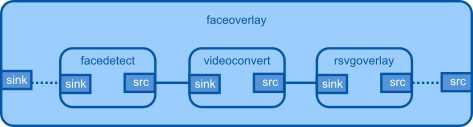
\includegraphics[width=1.0\textwidth]{../images/faceoverlay-design.png}\par
  \caption{Simplificación de diagrama del elemento \textit{gstfaceoverlay}.}
    \label{fig:faceoverlay-design}
  \caption*{Fuente: Autoría propia}
\end{figure}

\begin{figure}[!h]
  \centering
    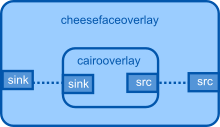
\includegraphics{../images/cheesefaceoverlay-design.png}\par
  \caption{Simplificación de diagrama del elemento \textit{gstcheesefaceoverlay}.}
    \label{fig:cheesefaceoverlay-design}
  \caption*{Fuente: Autoría propia}
\end{figure}

\section{Capabilities}
Debido a que este elemento es en términos prácticos una herencia de (en realidad
un \textit{bin} que contiene a \textit{gstcairooverlay}), este dispone de
un único \textit{sink pad} y único \textit{src pad} los cuales están disponibles
siempre. Además tanto los formatos de imagen que acepta y que genera como salida
son \textit{BGRx}, \textit{BGRA}, \textit{RGB16}. La descripción completa
respecto a las plantillas de sus \textit{pad} mostrada según el comando
\framebox{\textit{gst-inspect-1.0 cheesefaceoverlay}} se muestra a continuación:

\begin{verbatim}
Pad Templates:
  SINK template: 'sink'
    Availability: Always
    Capabilities:
      video/x-raw
                 format: { (string)BGRx, (string)BGRA, (string)RGB16 }
                  width: [ 1, 2147483647 ]
                 height: [ 1, 2147483647 ]
              framerate: [ 0/1, 2147483647/1 ]
  
  SRC template: 'src'
    Availability: Always
    Capabilities:
      video/x-raw
                 format: { (string)BGRx, (string)BGRA, (string)RGB16 }
                  width: [ 1, 2147483647 ]
                 height: [ 1, 2147483647 ]
              framerate: [ 0/1, 2147483647/1 ]
\end{verbatim}


\section{Propiedades}
Las propiedades de este objeto es una sola:
\begin{center}
  \begin{longtable}{| p{.2\textwidth} | p{.2\textwidth} | p{.6\textwidth} |}
  \hline

  % Cabecera
  \textbf{Propiedad} &
  \textbf{Tipo} &
  \textbf{Descriptión de la propiedad}
  \\ \hline

  % Fila
  \textbf{location} &
  \textit{string} &
  Es la ubicación (ruta) del archivo en formato \textit{JSON} que representa un
  \textit{sprite}
  \\ \hline

  % Fila
  \textbf{data} &
  \textit{string} &
  Es una cadena de carácteres que sigue la estructura de un \textit{sprite}.
  Puede ser visto como el contenido del archivo \textit{JSON}.
  \\ \hline
  \end{longtable}
\end{center}

\section{Sprite}
Con el fin de generar una animación a partir de imágenes estáticas, se ha ideado
una clase que además es representada en una estructura en formato \textit{JSON}.
Esta estructura sirve para que \textit{gstcheesefaceoverlay} pueda saber en que
coordenadas en píxeles, en qué escala, durantes cuántos cuadros y para qué
personas colocar las imágenes. Ello permite crear animaciones complejas y
buenas visualmente. Este archivo \textit{JSON} es deserializado por
el filtro en un objeto llamado \textit{CheeseMultifaceSprite}, el cual a su vez
contiene otros objetos, los cuales se describen a continuación:\\

\subsection{CheeseFaceSpriteFrame}
Representa una imagen estática (la cual se almacena en un \textit{buffer} de
píxeles) con una duración. A continuación se lista las propiedades del objeto
que están representadas también en formato \textit{JSON}:

\begin{center}
  \begin{longtable}{| p{.2\textwidth} | p{.2\textwidth} | p{.6\textwidth} |}
  \hline

  % Fila
  \textbf{Propiedad} &
  \textbf{Tipo} &
  \textbf{Descriptión de la propiedad}
  \\ \hline

  % Fila
  \textbf{duration} &
  \textit{unsigned int} &
  Es el número de frames durante el cual la imagen será mostrada.
  \\ \hline

  % Fila
  \textbf{location} &
  \textit{string} &
  La ruta del archivo de la imagen.
  \\ \hline

  % Fila
  \textbf{base-scale-factor} &
  \textit{string} &
  El factor por el cual se escalará la imagen. \textit{gstcheesefaceoverlay}
  escala las imágenes con dos factores: el primer factor es respecto al tamaño
  del \textit{bounding box} del rostro y el segundo es este factor.
  \\ \hline
  \end{longtable}
\end{center}

En \textit{JSON}, esta estructura podría ser representada de la siguiente
manera:\\
\begin{verbatim}
{
    "base-scale-factor": 1.2,
    "duration": 80,
    "location": "/home/cfoch/Pictures/sprite/head/3.png"
}
\end{verbatim}

Lo cual significa que la imagen en la ubicación
\textit{/home/cfoch/Pictures/sprite/head/3.png} será renderizada desde solo por
una duración de 80 frames. La escala de esta imagen se aplica primero escalando
al mismo tamaño del \textit{bounding box} y luego multiplicando por el factor de
escala base.\\

\subsection{CheeseFaceSpriteKeypoint}
Representa una animación para un punto específico \textit{key point} de una
cara. Es un conjunto de \textit{CheeseFaceSpriteFrame}. Lo que significa que una
vez terminada la duración de un \textit{CheeseFaceSpriteFrame} se muestra la
imagen del siguiente \textit{CheeseFaceSpriteFrame}. Así sucesivamente, hasta
que la duración total se agote. La animación puede repetirse indefinidamente si
así se indica.

\begin{center}
  \begin{longtable}{| p{.2\textwidth} | p{.2\textwidth} | p{.6\textwidth} |}
  \hline

  % Fila
  \textbf{Propiedad} &
  \textbf{Tipo} &
  \textbf{Descriptión de la propiedad}
  \\ \hline

  % Fila
  \textbf{keypoint} &
  \textit{CheeseFaceKeypoint} &
  Es el tipo de punto facial del cual este objeto representará la animación.
  \\ \hline

  % Fila
  \textbf{rotate} &
  \textit{boolean} &
  Si es verdadero, indica que la imagen debe rotar en la orientación del ángulo
  formado por los ojos. Si es falso, la imagen no debe rotarse.
  \\ \hline

  % Fila
  \textbf{loop} &
  \textit{boolean} &
  Si es verdadero, una vez culminada la duración se vuelve a mostrar la imagen
  del primer \textit{CheeseFaceSpritFrame} en la lista y se continúa de esta
  manera indefinidamente. Si es falso, una vez culminada la duración total, no
  se mostrará una sola imagen más.
  \\ \hline
  \end{longtable}
\end{center}

En \textit{JSON}, esta estructura podría ser representada de la siguiente
manera:\\

\begin{verbatim}
"head": {
    "rotate": true,
    "loop": true,
    "frames": [
        {
            "base-scale-factor": 1.2,
            "duration": 80,
            "location": "/home/cfoch/Pictures/sprite/head/3.png"
        },
        {
            "base-scale-factor": 1.2,
            "duration": 20,
            "location": "/home/cfoch/Pictures/sprite/head/2.png"
        }
    ]
}
\end{verbatim}

\textit{``frames''} representa la lista de
\subsection{CheeseFaceSpriteKeypoint}. Lo cual significa que en la posición de
la cabeza, desde que un rostro se detecta, los primeros 80 cuadros, se mostrará
la imagen en \textit{/home/cfoch/Pictures/sprite/head/3.png} y los siguientes 20
cuadros se mostrará la imagen en
\textit{/home/cfoch/Pictures/sprite/head/2.png}. Si la cara rota frente a la
cámara, la imagen rotará en su misma orientación (según el ángulo formado por 
sus ojos).

Los puntos faciales disponibles se describen en la siguiente tabla:
\begin{center}
  \begin{longtable}{| p{.55\textwidth} | p{.2\textwidth} | p{.25\textwidth} |}
  \hline

  % Fila
  \textbf{En \textit{C}} &
  \textbf{Representación en \textit{JSON}} &
  \textbf{Descripción}
  \\ \hline

  % Fila
  \textit{CHEESE\_FACE\_KEYPOINT\_PHILTRUM} &
  \textit{philtrum} &
  Representa el filtrum (zona de la cara entre nariz y labio superior).
  \\ \hline

  % Fila
  \textit{CHEESE\_FACE\_KEYPOINT\_MOUTH} &
  \textit{mouth} &
  Representa el centro de la boca.
  \\ \hline

  % Fila
  \textit{CHEESE\_FACE\_KEYPOINT\_LEFT\_EYE} &
  \textit{left-eye} &
  Representa el centro del ojo izquiedo.
  \\ \hline

  % Fila
  \textit{CHEESE\_FACE\_KEYPOINT\_RIGHT\_EYE} &
  \textit{right-eye} &
  Representa el centro del ojo derecho.
  \\ \hline

  % Fila
  \textit{CHEESE\_FACE\_KEYPOINT\_NOSE} &
  \textit{nose} &
  Representa la posición de la punta de la nariz.
  \\ \hline

  % Fila
  \textit{CHEESE\_FACE\_KEYPOINT\_LEFT\_EAR} &
  \textit{left-ear} &
  Representa la zona de la oreja izquierda. Una imagen colocada sobre este
  punto, tendrá su zona lateral centrada en tal punto.
  \\ \hline

  % Fila
  \textit{CHEESE\_FACE\_KEYPOINT\_RIGHT\_EAR} &
  \textit{right-ear} &
  Representa la zona de la oreja derecha. Una imagen colocada sobre este punto,
  tendrá su zona lateral centrada en tal punto.
  \\ \hline

  % Fila
  \textit{CHEESE\_FACE\_KEYPOINT\_FACE} &
  \textit{face} &
  Representa el centro del rostro.
  \\ \hline

  % Fila
  \textit{CHEESE\_FACE\_KEYPOINT\_HEAD} &
  \textit{head} &
  Representa la zona de la cabeza. Una imagen colocada sobre este punto,
  tendrá su zona inferior centrada en tal punto.
  \\ \hline
  \end{longtable}
\end{center}

\subsection{CheeseFaceSprite}
Un objeto de este tipo tiene un conjunto de \textit{CheeseFaceSpriteFrame}. Por
tanto, este representa el conjunto de animaciones por cada punto facial para un
rostro en específico.

En \textit{JSON}, esta estructura podría ser representada de la siguiente
manera:\\

\begin{verbatim}
{
    "head": {
        "rotate": true,
        "loop": true,
        "base-scale-factor": 0.5,
        "frames": [
            {
                "base-scale-factor": 1.2,
                "duration": 80,
                "location": "/home/cfoch/Pictures/sprite/head/3.png"
            },
            {
                "base-scale-factor": 1.2,
                "duration": 20,
                "location": "/home/cfoch/Pictures/sprite/head/2.png"
            }
        ]
    },
    "philtrum": {
        "rotate": true,
        "loop": true,
        "base-scale-factor": 0.5,
        "frames": [
            {
                "base-scale-factor": 0.5,
                "duration": 20,
                "location": "/home/cfoch/Pictures/sprite/philtrum/2.png"
            }
        ]
    }
}
\end{verbatim}

Lo cual significa que el rostro tendrá animaciones en la zona de su cabeza y
filtrum, según lo explicado en la subsección anterior.

\subsection{CheeseFaceMultiSprite}
Un objeto de este tipo tiene un conjunto de \textit{CheeseFaceSprite}. Por lo
que este representa el conjunto de animaciones para múltiples rostros en
los puntos faciales especificados. \textbf{Este es el formato aceptado por
\textit{gstcheesefaceoverlay}}.

En \textit{JSON}, esta estructura podría ser representada de la siguiente
manera:\\

\begin{verbatim}
[
    {
        "philtrum": {
            "rotate": true,
            "loop": true,
            "base-scale-factor": 0.5,
            "frames": [
                {
                    "base-scale-factor": 0.5,
                    "duration": 5,
                    "location": "/home/cfoch/Pictures/sprite/philtrum/2.png"
                }
            ]
        },
        "left-eye": {
            "rotate": true,
            "loop": true,
            "base-scale-factor": 0.5,
            "frames": [
                {
                    "base-scale-factor": 0.5,
                    "duration": 5,
                    "location": "/home/cfoch/Pictures/sprite/eye/1.png"
                },
                {
                    "base-scale-factor": 0.5,
                    "duration": 10,
                    "location": "/home/cfoch/Pictures/sprite/eye/2.png"
                }
            ]
        },
        "right-eye": {
            "rotate": true,
            "loop": true,
            "base-scale-factor": 0.5,
            "frames": [
                {
                    "base-scale-factor": 0.5,
                    "duration": 5,
                    "location": "/home/cfoch/Pictures/sprite/eye/1.png"
                },
                {
                    "base-scale-factor": 0.5,
                    "duration": 10,
                    "location": "/home/cfoch/Pictures/sprite/eye/2.png"
                }
            ]
        },
        "head": {
            "rotate": true,
            "loop": true,
            "base-scale-factor": 0.5,
            "frames": [
                {
                    "base-scale-factor": 1.2,
                    "duration": 20,
                    "location": "/home/cfoch/Pictures/sprite/head/1.png"
                }
            ]
        }
    },
    {
        "head": {
            "rotate": true,
            "loop": true,
            "base-scale-factor": 0.5,
            "frames": [
                {
                    "base-scale-factor": 1.2,
                    "duration": 80,
                    "location": "/home/cfoch/Pictures/sprite/head/3.png"
                },
                {
                    "base-scale-factor": 1.2,
                    "duration": 20,
                    "location": "/home/cfoch/Pictures/sprite/head/2.png"
                }
            ]
        },
        "philtrum": {
            "rotate": true,
            "loop": true,
            "base-scale-factor": 0.5,
            "frames": [
                {
                    "base-scale-factor": 0.5,
                    "duration": 20,
                    "location": "/home/cfoch/Pictures/sprite/philtrum/2.png"
                }
            ]
        }
    }
]
\end{verbatim}

Como se puede observar acá se detalla la animación de dos rostros. El primer
rostro tiene animaciones asignadas a su filtrum, ojo izquierdo, ojo derecho y
cabeza. El segundo rostro tiene animaciones asignadas a solamente su cabeza y
philtrum.

\section{Ejemplos de \textit{pipelines}}
Existe una lista muy grande de \textit{pipelines} que se pueden formar con este
filtro. Se muestra algunos ejemplos sencillos:

Desde la cámara web:
\begin{verbatim}
$ gst-launch-1.0 v4l2src ! videoconvert ! \
  cheesefacetrack scale-factor=0.5 \
  landmark=shape_predictor_68_face_landmarks.dat ! \
  videoconvert ! cheesefaceoverlay location=sprite.json ! \
  videoconvert ! xvimagesink
\end{verbatim}

Desde un archivo de video:
\begin{verbatim}
$ gst-launch-1.0 filesrc location=archivo.ogv ! \
  decodebin ! videoconvert ! \
  cheesefacetrack scale-factor=0.5 \
  landmark=shape_predictor_68_face_landmarks.dat ! \
  videoconvert ! cheesefaceoverlay location=sprite.json ! \
  videoconvert ! xvimagesink
\end{verbatim}

\section{Resultado esperado: medición latencia por \textit{buffer}}
En esta sección se muestra los resultados de la medición de latencia en ciertos
\textit{pipelines} que usan \textit{gstcheesefaceoverlay}. También se mide la
latencia de \textit{pipelines} similares usando \textit{gstfaceoverlay} con el
objetivo de hacer una comparación. La herramienta principal que se usa para
medir la latencia es el subsistema de rastreo (\textit{tracing}) de
\textit{GStreamer}.

\chapter{Integración de ambos filtros en Cheese}
En este capítulo se desarrolla el cuarto objetivo el cual comprende el diseño
de una interfaz gráfica para los filtros desarrollados en \textit{Cheese}. Para
cumplir este objetivo, el primer paso fue desarrollar un mockup. Luego se diseñó
diagramas de clases y secuencias con la finalidad de tener una interfaz gráfica
a futuro que no solo permita efectos del tipo a los realizados en
\textit{gstcheesefaceoverlay}, sino que se pueda extender a aplicación a tener
una librería donde se sobrepongan imágenes estáticas sin el uso de visión
artificial o filtros más complicados que permitan cargar modelos en 3D para
sobreponerlos de manera similar a como aplicaciones como \textit{Snapchat} y
\textit{Facebook} soportan actualmente. Finalmente, ya que
\textit{gstcheesefacetrack} y \textit{gstcheesefacedetect} dependen de un
modelo entrenado para detectar los puntos faciales del rostro se tuvo que
modificar el diáologo de preferencias de \textit{Cheese} para que permita
al usuario seleccionar entre el modelo que \textit{dlib} incluye por defecto o
cualquier otro. Como se mencionó, \textit{Cheese} está escrito en Vala, y por
ello se usó este lenguaje. Además se tuvo que crear una \textit{API} que
permite usar el código escrito en \textit{C} (para el objetivo específico 2) en
Vala.

\section{Mock-up}
El primer paso fue desarrollar el \textit{mock-up} de la interfaz gráfica. Véase
la figura \ref{fig:cheese-mockup}. En la figura se aprecia un botón sobre la
cabecera (\textit{header bar} o área de título) de la ventana principal de
\textit{Cheese}. Al hacer clic en tal botón, se debe mostrar un \textit{pop-up}
donde se muestre una grilla de imágenes. Cada imagen representa un
\textit{sprite} (un \textit{CheeseFaceSprite}). Internamente, \textit{Cheese}
debe construir un \textit{CheeseMultifaceSprite} en el orden de la selección. Al
hacer clic en el botón con el ícono del visto bueno, el filtro de sobreposición
de imágenes debería aplicarse sobre el \textit{viewport} de Cheese.\\

\begin{figure}[!h]
  \centering
    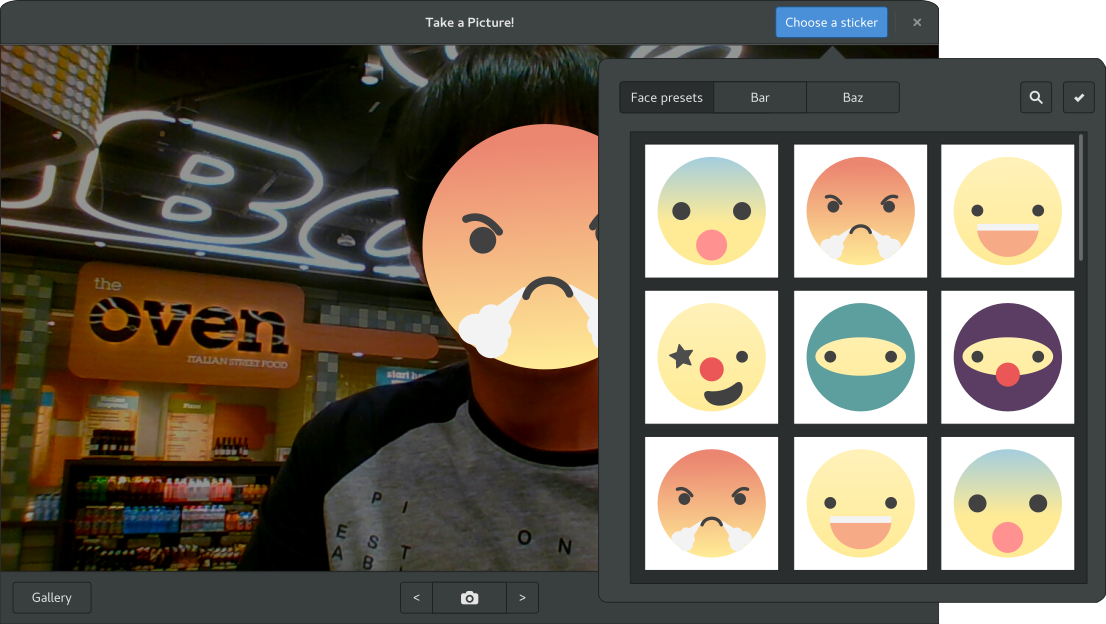
\includegraphics[width=1.0\textwidth]{../images/cheese-mockup.png}\par
  \caption{Mock-up de interfaz gráfica para \textit{gstcheesefaceoverlay}. Las
    imágenes de emoticonos que se muestran son solo referenciales. La parte
    inferior de la imagen fue una idea propuesta por Allan Day, y no se ha
    desarrollado pues no formaba parte del objetivo.}
    \label{fig:cheese-mockup}
  \caption*{Fuente: Autoría propia y basado en un \textit{mock-up} desarrollado
    por Allan Day y otros archivos del repositorio en \textit{git} de
    \textit{mock-ups} del \textit{GNOME Design Team}. Los emoticonos son parte
    de Antü Plasma Suite y diseñados por Fabián Alexis.}
\end{figure}

\section{Archivos \textit{.sprite} para \textit{face presets}}
Según la especificación de \textit{freedesktop.org} (un proyecto creado para la
interoperabilidad entre entornos de escritorio para \textit{UNIX} y
\textit{Linux}), los archivos de \textbf{datos} deben colocarse relativos a un
directorio base a la variable de entorno \textit{\$XDG\_DATA\_DIRS}
\cite{freedesktopXDGBase}. Para este objetivo, se ha escogido guardar los
archivos de extensión \textit{.sprite} en la ruta
\textit{\$XDG\_DATA\_DIRS/cheese/sprites/face-presets}.\\

Los archivos de extensión de \textit{.sprite} en tal ruta representan un
\textit{CheeseFaceSprite} y son archivos ``key files'' que su sintaxis sigue
también la especificación \textit{Desktop Entry Specification} de la
\textit{freedesktop.org} \cite{freedesktopDesktopEntrySpec}. Un ejemplo de este
archivo puede ser:\\

\begin{verbatim}
[Face]
Name=Face Test Sprite
Location=/usr/share/cheese/stickers/sprites/face-presets/face1.json
Thumbnail=/usr/share/cheese/stickers/sprites/face-presets/thumbnails/face1.png
\end{verbatim}

La clave ``Location'' representa la ubicación del archivo de \textit{sprite}
\textit{.json} aceptado por \textit{gstcheesefaceoverlay}. Cuando
\textit{Cheese} lea este archivo usará el valor en ``Location'' para ``decirle''
a \textit{gstcheesefaceoverlay} que renderice las imágenes a sobreponer según
ese archivo. Luego, la clave ``Thumbnail'' representa la imagen que se muestra
como vista previa en el \textit{grid} que se explicará en la siguiente sección.\\

\textit{Cheese} puede distribuir su propio conjunto de ``sprites'' pero ya que
se usa el directorio base \textit{\$XDG\_DATA\_DIRS}, los usuarios podrían
definir sus propios \textit{sprites} sin tener que modificar el directorio de
instalación de \textit{Cheese}.

\section{Diagrama de clases}
El diagrama de clases (figura \ref{fig:diagrama-clases}) se ha diseñado pensando
en tener una interfaz que sea extendible a futuro. Cada clase que empieza con
\textit{Cheese} significa que está dentro de tal \textit{namespace}.\\

\textit{CheeseStickerGrid} es una clase heredada del \textit{widget}
\textit{Gtk.FlowBox} que representa un contenedor (en formal de grilla) de
botones (el atributo \textit{button} es solo representativo) del tipo
\textit{CheeseStickerButton}. Además dispone de un atributo
\textit{filter\_func} el cual representa la función de búsqueda en caso el
\textit{widget} soporte la búsqueda. Luego se tiene un método
\textit{load\_buttons} el cual las clases que hereden de esta deberán
sobreescribir. Por ejemplo, en este proyecto, como se ve en la figura
\ref{fig:cheese-mockup} los botones a cargar serían los archivos
\textit{.sprite} que están localizados en
\textit{\$XDG\_DATA\_DIRS/cheese/sprites/face-presets}. Si tuviéramos archivos
similares a los \textit{.sprite} que describan filtros en 3D, entonces bastaría
con crear otra clase que herede de esta y que cargue los archivos necesarios.\\

\textit{CheeseStickerButton} es una clase que hereda del \textit{widget}
\textit{Gtk.ToggleButton} al cual se le aplica un estilo CSS para que el botón
se vea grande y de forma cuadrada. Esta clase solo representa un botón con una
imagen. Al heredar \textit{CheeseFacePresetButton} de
\textit{CheeseStickerButton} este botón puede guardar información del archivo
\textit{sprite} en el atributo \textit{face\_sprite\_json}. La manera de crear
un botón \textit{CheeseFacePresetButton} es mediante una llamada al método
estático \textit{new\_from\_keyfile}.\\

\begin{figure}[!h]
  \centering
    
\includegraphics{../images/cheese-mockup-face-preset-button.png}\par
  \caption{Representación de \textit{{CheeseFacePresetButton}}}
    \label{fig:cheese-sticker-button}
  \caption*{Fuente: el emoticón es parte de Antü Plasma Suite y ha sido
    diseñado por Fabián Alexis.}
\end{figure}

\textit{CheeseFacePresetGrid} como se mencionó, hereda de
\textit{CheeseStickerGrid}. Este además implementa una interfaz
\textit{CheeseStickerPageIFace} y un \textit{CheeseFaceGridInterface}. La
primera interfaz es útil para que a partir de unos botones seleccionados se
cree un \textit{Cheese.Effect} (el cual representa un efecto o filtro) y además
es útil también porque provee señales (\textit{Signals}) que se emiten cada vez
que es posible crear un efecto (por ejemplo si se seleccionaron 1 o más botones)
o si no es posible (si no hay botón seleccionado) para habilitar o deshabilitar
el botón de ''visto bueno`` como se puede ver en la figura
\ref{fig:cheese-mockup}.\\

\begin{figure}[!h]
  \centering
    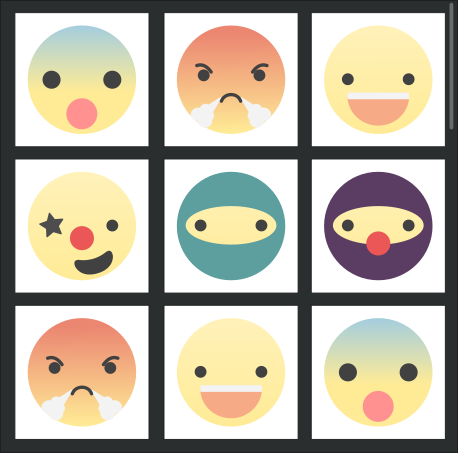
\includegraphics{../images/cheese-mockup-face-preset-grid.png}\par
  \caption{Representación de \textit{{CheeseFacePresetGrid}}}
    \label{fig:cheese-sticker-button}
  \caption*{Fuente: Autoría propia y basado en archivos del repositorio en
    \textit{git} de \textit{mock-ups} del \textit{GNOME Design Team}. Los
    emoticonos son parte de Antü Plasma Suite y diseñados por Fabián Alexis.}
\end{figure}

Finalmente, \textit{CheeseStickersPopup} representa el \textit{pop-up} que se
muestra cada vez que se hace clic en el botón azul de la barra de título. Este
dispone de métodos de retrollamada para realizar la acción de aplicar el efecto
o de buscar un efecto (o filtro) cuando se hace clic en el botón del ''visto
bueno`` o cuando se realiza una búsqueda, respectivamente. Un pop-up de este
tipo puede contener varios \textit{widgets} que implementen
\textit{CheeseFaceGridInterface}.

\afterpage{
    \clearpage
    \KOMAoptions{paper=A3}
    \addtolength{\hoffset}{-1.50cm}
    \recalctypearea
    \begin{figure}
      \centering
      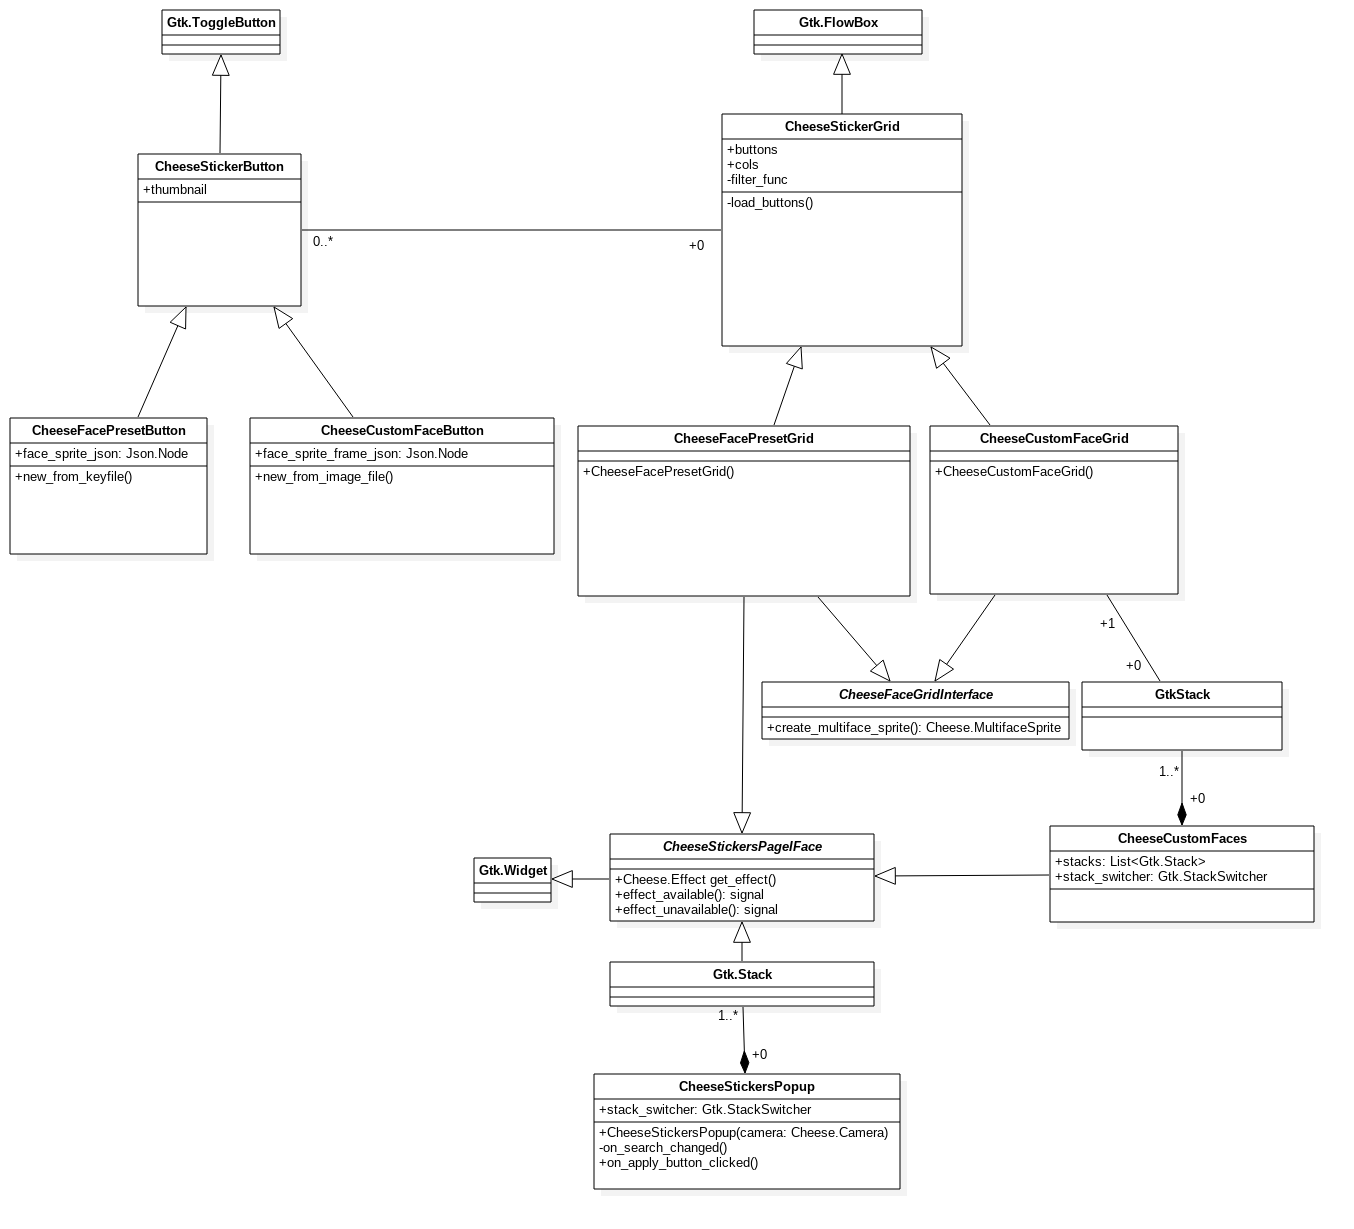
\includegraphics[width=1.2\textwidth]{../images/diagrama-clases.png}\par
      \caption{Diagrama de clases de interfaz gráfica para
        \textit{gstcheesefaceoverlay} en \textit{Cheese}. Las clases
        \textit{CheeseCustomFaceGrid}, \textit{CheeseCustomFaceButton} y
        \textit{CheeseCustomFaces} no se han implementado, pues está fuera del
        alcance.}
      \label{fig:diagrama-clases}
      \caption*{Imagen de autoría propia}
    \end{figure}
    \clearpage
    \KOMAoptions{paper=A4,pagesize}
    \recalctypearea
}

\section{Diagrama de secuencias}
El diagrama de secuencias (figura \ref{fig:diagrama-secuencias}) representa el
flujo de la interacción entre el usuario y el \textit{pop-up} agregado en
\textit{Cheese}. El flujo inicia cuando el usuario hace clic en el botón
``Choose a sticker''. Al hacer clic, el bucle principal de \textit{GLib} recibe
el evento y se crea y muestra un \textit{pop-up} sobre la ventana de
\textit{Cheese}. Al momento de la creación de un \textit{CheeseStickersPopup}
se crea además un \textit{CheeseFacePresetsGrid} el cual a su vez crea botones
como tantos archivos \textit{sprite} existan en
\textit{\$XDG\_DATA\_DIRS/cheese/sprites/face-presets}.\\

Una vez cargado el \textit{pop-up}, el botón del icono de ``visto bueno'' está
desactivado. Apenas el usuario hace clic en uno los botones en la grilla, una
señal \textit{``effect-available''} es emitida de tal modo que activa el botón
del icono de ``visto bueno''. Si se deseleccionan todos los botones, se emite la
señal \textit{``effect-unavailable''} y el botón es desactivado.\\

Finalmente, al hacer clic en el botón del ``visto bueno'', internamente,
se construye un \textit{sprite} en un formato aceptado por
\textit{gstcheesefaceoverlay} en el orden de la selección. De no haber ningún
problema, se aplica el efecto y se muestra en el \textit{viewport} de \textit{Cheese}.
De haberlo, se muestra un \textit{GtkInfoBar} que avisa que hubo un error.

\afterpage{
    \clearpage
    \KOMAoptions{paper=A3}
    \addtolength{\hoffset}{-1.00cm}
    \recalctypearea
    \begin{figure}
      \centering
      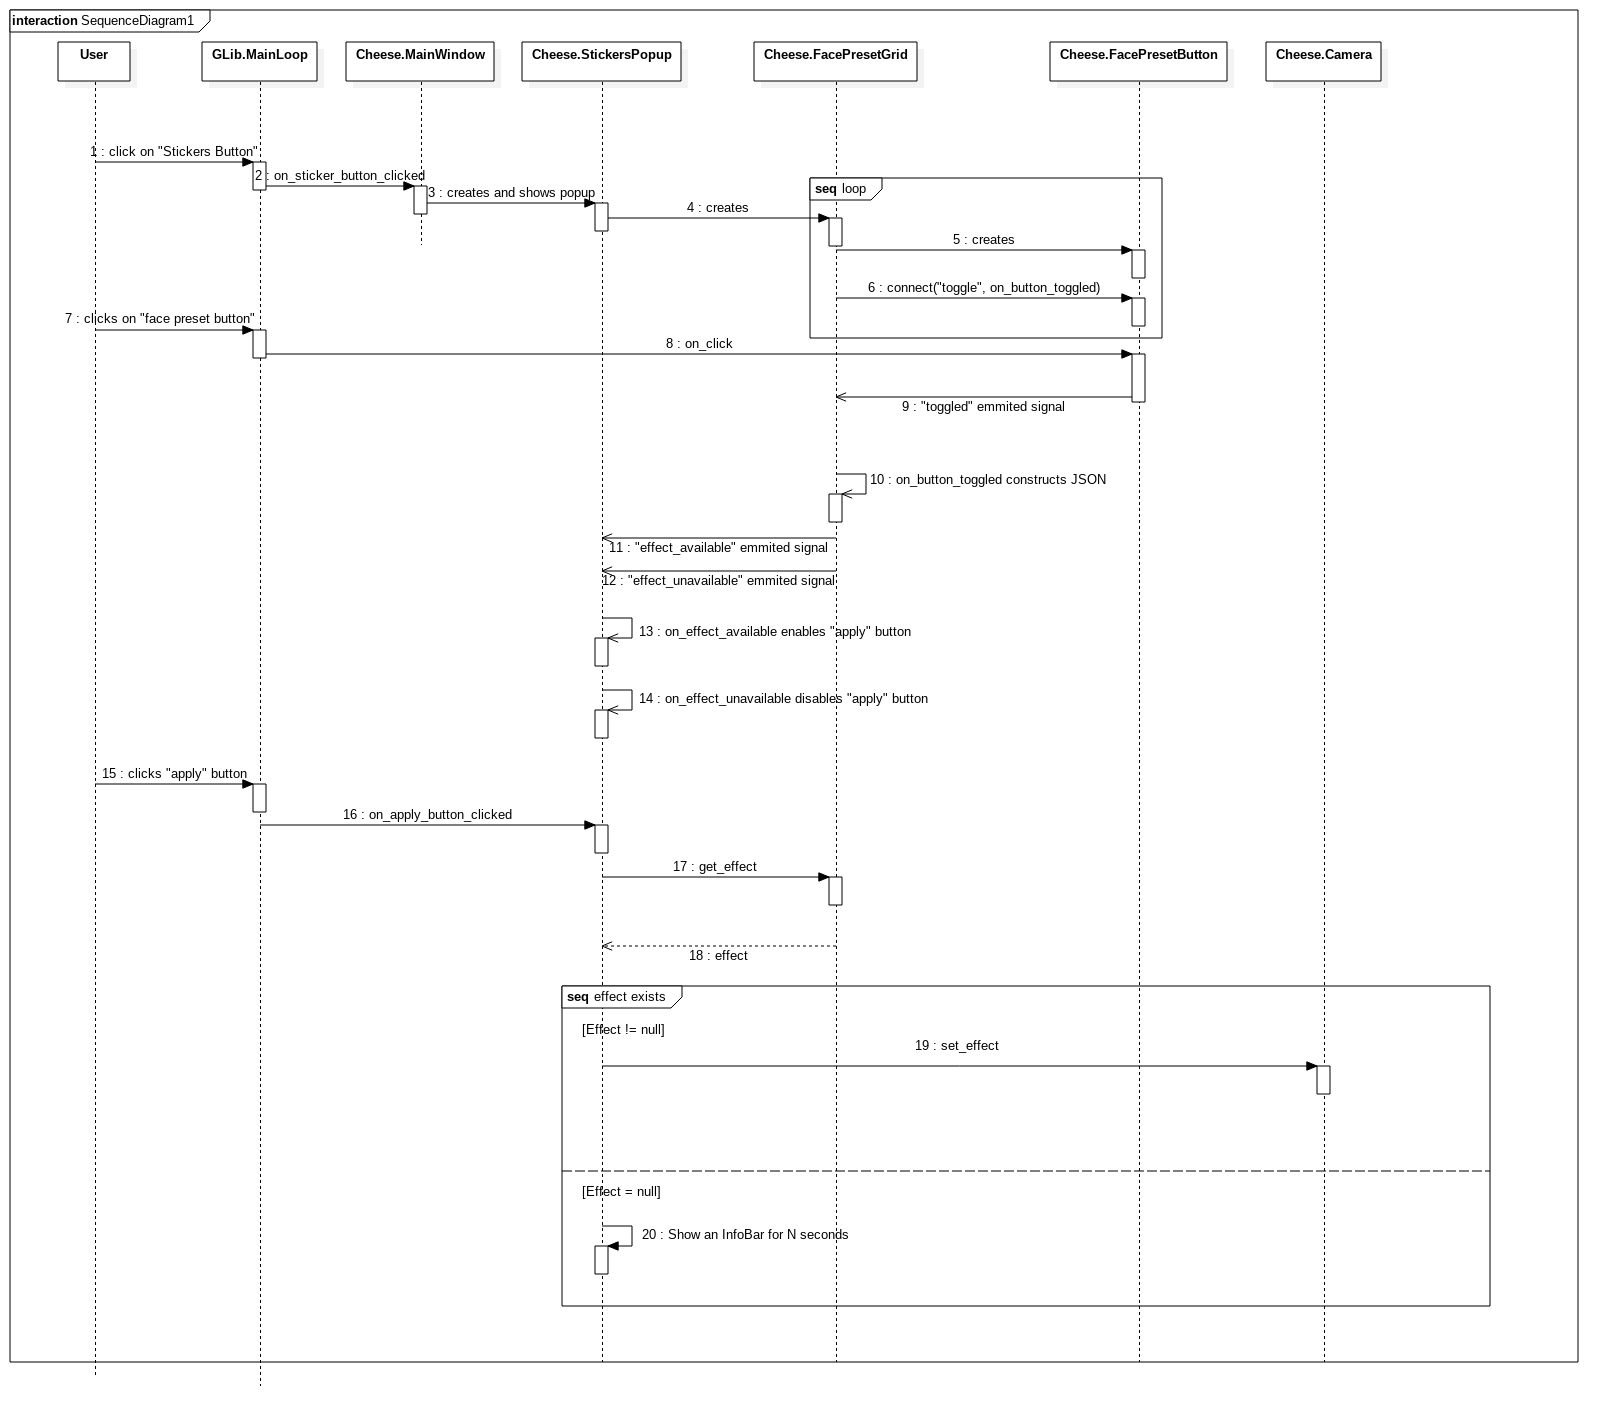
\includegraphics[width=1.2\textwidth]{../images/diagrama-secuencias.png}\par
      \caption{Diagrama de secuencias.}
      \label{fig:diagrama-secuencias}
      \caption*{Imagen de autoría propia}
    \end{figure}
    \clearpage
    \KOMAoptions{paper=A4,pagesize}
    \recalctypearea
}

\chapter{Conclusiones y trabajos futuros}
\section{Conclusiones}
\subsection{Trabajos futuros}

\bibliographystyle{apacite}
\bibliography{references}{}


\end{document}
